\documentclass[10pt,a4paper]{article}
\usepackage[margin=2.0cm]{geometry}
\usepackage{amsmath}
\usepackage{graphicx}
\usepackage{longtable,booktabs,pdflscape}
\usepackage{url}
\usepackage[hidelinks]{hyperref}
\usepackage{fontspec}
\setmainfont{DejaVu Serif}
\setmonofont{DejaVu Sans Mono}[Scale=0.85]
\setlength{\parskip}{4pt}
\setlength{\parindent}{0pt}
\setlength{\emergencystretch}{3em}
\graphicspath{{./}}
\begin{document}
\title{v7 cloning campaign: subset generation, pre-training, in-sample optimization and held-out generalization}
\author{}\date{2026-09-09}
\maketitle


State of the results on 2026-09-09 (revised report; the first version was dated 2026-09-08). Every number in this report is read from a file of the pulled runs (\path{~/Documents/Research/xcquinox-results/runs/dfs_step7/}) or from a CSV the figure suite wrote beside the figure it belongs to; the file is named at each table. The figures are the tracked sets under \path{notebooks/analysis/figures_dfs_step7_*}; the validation-best checkpoint channel is used for every optimization figure unless a caption says otherwise. Each figure is described panel by panel with the values it shows, so that the text can be read without magnifying the figure.

The sections follow the pipeline: the model and its descriptors (Sec. 1), the generation of the training subsets, which is the step before any network is fitted (Sec. 2), the pre-training of each architecture to its parent functional (Sec. 3), the optimization on the training subsets read on the training data itself (Sec. 4), and the held-out generalization (Sec. 5); the pending items close the document (Sec. 6).

\section*{Scope and inventory}

The v7 campaign trains one network pair (an exchange network and a correlation network) per architecture and per training-subset size, under one protocol, on the cluster as separate runs that differ in their architecture axis. Each run carries its own pre-training (the cloning of the parent functional), a fidelity certificate that gates its training array, and the array itself, one cell per (architecture, subset size). The figures and tables of this report are drawn once over every finished cell of every run: the runs are merged into one view (\path{family_runs.yaml}, \path{merge_family_runs.py}; the runbook's v7 section) and the architecture axis is the one of Sec. 1.5, with the run of each cell recorded in the tables' first column. The architecture names are those of Sec. 1.5.

\begin{landscape}
\begin{small}
\begin{longtable}{lp{0.320\linewidth}p{0.320\linewidth}l}
\toprule Run & Architectures & Cells done / planned & Run directory \\ \midrule \endhead
size & deep\_3x16, deep\_attn\_3x16 & deep\_3x16 11/11, deep\_attn\_3x16 9/11 & \path{run_20260902T145245Z} \\
families & deep0\_3x16, deep0\_attn\_3x16, deep0\_cusp\_3x16 & deep0\_3x16 11/11, deep0\_attn\_3x16 2/11, deep0\_cusp\_3x16 0/11 & \path{run_20260902T145247Z} \\
meta-GGA families & deep0\_cusp\_mgga\_3x16, deep0\_mgga\_3x16, deep0\_mgga\_attn\_3x16, deep0\_rung35\_mgga\_3x16, deep0\_rung35ms\_mgga\_3x16 & 0/55 (the first certificate reads FAIL, Sec. 3.6; the other four are pending) & \path{run_20260902T145250Z} \\
25-cycle arm & deep\_3x16, tag \texttt{[25 cycles]} & 0/5 (pre-training done, training queued) & \path{run_20260908T153856Z} \\
dpyscf-parity arm & deep\_3x16, tag \texttt{[dpyscf parity]} & 0/5 (pre-training done, training queued) & \path{run_20260908T153908Z} \\
\bottomrule \end{longtable}
\end{small}
\end{landscape}


The subset-size axis is 1, 2, 3, 4, 5, 6, 7, 12, 15, 18 and 26 training points, drawn from the 26-point DFS training pool by the Jensen-Shannon subset selection of Sec. 2; the membership of every subset is in the table of Sec. 2.4. Basis 6-311++G(3df,2pd), grid level 3, density fitting on, for every stage (\path{fidelity_certificate.json}, keys \path{basis}, \path{grid_level}, \path{density_fit}). The cells that have not finished are the attention and cusp architectures at the larger subsets and the whole meta-GGA group; they appear as "pending" in the tables below and are absent from the figures. Two arms of a follow-up (the 25-cycle SCF arm and the dpyscf-parity arm, both on the deep\_3x16 architecture) were submitted on 2026-09-08 and carry no results yet.

\section*{1. Model, descriptors and the functional form}

Sources: \path{xcquinox/alec/networks.py} (the two networks), \path{xcquinox/alec/descriptors.py} and \path{xcquinox/alec/metagga.py} (the extra descriptors), \path{xcquinox/net.py} (the attention block), \path{xcquinox/alec/config.py} (the architecture registry). The coordinate convention is the DFS one (\texttt{model.descriptor\_coordinates: dfs} in every v7 file), following Dick and Fernandez-Serra, PRB 104, L161109 (2021), whose equation numbers are quoted as "DFS Eq. n".

\subsection*{1.1 Density variables}

With $n = n_\alpha + n_\beta$ the total density and $\sigma = |\nabla n|^2$,

\[
k_F = (3\pi^2 n)^{1/3}, \qquad
s = \frac{|\nabla n|}{2 k_F n}, \qquad
r_s = \left(\frac{3}{4\pi n}\right)^{1/3}, \qquad
\zeta = \frac{n_\alpha - n_\beta}{n}, \qquad
\phi(\zeta) = \tfrac12\left[(1+\zeta)^{4/3} + (1-\zeta)^{4/3}\right].
\]

$s$ is the reduced density gradient (DFS Eq. 5), $\phi$ the spin-scaling factor of DFS Eq. 4 ($\phi = 1$ at $\zeta = 0$, $2^{1/3}$ at full polarization). The density is floored at the network's \path{lower_rho_cutoff} before any of these is formed.

\subsection*{1.2 Network coordinates (DFS coordinates)}

The exchange network reads one coordinate at the GGA level and two at the meta-GGA level; the correlation network reads three and four. They are logarithmic compressions of the variables above (DFS Eqs. 7 to 10):

\[
x_0 = \ln\!\left(n^{1/3} + 10^{-5}\right), \qquad
x_1 = \ln \phi(\zeta), \qquad
x_s = \left(1 - e^{-s^2}\right)\ln(s + 1), \qquad
x_\alpha = \ln\frac{\alpha + 1}{2}.
\]

Exchange input: $[x_s, \ldots]$, where $s$ is that of the doubled spin channel $2 n_\sigma$ (the exchange network is evaluated per spin channel, Sec. 1.4). Correlation input: $[x_0, x_1, x_s, \ldots]$ on the total density. The ellipsis holds the extra descriptors of the architecture, in the registry's list order; on the meta-GGA rung the raw $\alpha$ column among them is replaced by $x_\alpha$.

\subsection*{1.3 Extra descriptors}

\textbf{Iso-orbital indicator (meta-GGA rung, \path{metagga})}, SCAN's $\alpha$ (Sun, Ruzsinszky and Perdew, PRL 115, 036402 (2015), Eq. 2; DFS Eq. 6):

\[
\alpha = \frac{\tau - \tau_W}{\tau_{\rm unif}}, \qquad
\tau = \tfrac12 \sum_i |\nabla\psi_i|^2 = \tfrac12 \sum_{\mu\nu} P_{\mu\nu}\, \nabla\chi_\mu\cdot\nabla\chi_\nu, \qquad
\tau_W = \frac{|\nabla n|^2}{8n}, \qquad
\tau_{\rm unif} = \tfrac{3}{10}(3\pi^2)^{2/3} n^{5/3}.
\]

$\tau$ is a contraction of the live one-particle density matrix $P$ against the AO gradients, so it is self-consistent and differentiable through the SCF without second derivatives. The bound $\alpha \ge 0$ (the von Weizsacker inequality) is imposed by a smooth positive part rather than a hard clip, so the descriptor and its derivative stay continuous where a spin channel holds one orbital.

\textbf{Nuclear cusp pair (\path{cusp})}, two bounded features per grid point:

\[
x_4 = \exp(-2 Z_{\rm nearest}\, r_{\min}), \qquad
x_5 = \tanh\!\left(\frac{1}{5}\ln \sum_A \frac{Z_A}{r_A}\right).
\]

$x_4$ is a proximity feature following the density-form cusp envelope $e^{-2Zr}$ (Steiner, J. Chem. Phys. 39, 2365 (1963), the density counterpart of Kato's wavefunction cusp); $x_5$ is the log-compressed bare-nuclear potential $-V_{\rm ext}$, the log and the $1/5$ scale being the conditioning of this work. Both are geometric, so the synthetic pre-training mesh (Sec. 3.1) carries no values for them.

The remaining registry descriptors (density-matrix statistics, the rung-3.5 occupancies) are not on any v7 axis and are not described here.

\subsection*{1.4 The functional form}

Each network is a multilayer perceptron with GELU activations, \path{depth} hidden layers of \path{nodes} units, a final linear layer (initialized at zero in the \path{deep_*} family, \path{zero_init_final_layer}), and an output squash. With $g$ the MLP output at a grid point,

\[
F_x = 1 + \mathcal{L}_{1.804}\!\left(G_x \cdot g_x\right), \qquad
F_c = 1 + \mathcal{L}_{2}\!\left(G_c \cdot g_c\right), \qquad
\mathcal{L}_{\lambda}(z) = \lambda\,\mathrm{sigmoid}\!\left(z - \ln(\lambda - 1)\right) - 1.
\]

$\mathcal{L}_\lambda(0) = 0$, so a zero MLP output returns $F = 1$ (the local density approximation), and $F$ stays in $(0, \lambda)$ for every $z$. $\mathcal{L}_\lambda$ is the DFS $I_a$ map (DFS Eq. 11) to machine precision. For exchange $\lambda = 1.804 = 1 + \kappa_{\rm PBE}$, the PBE Lieb-Oxford-motivated ceiling (PBE, PRL 77, 3865 (1996), Eq. 14); DFS uses 1.174 (the tighter bound of Perdew, Ruzsinszky, Sun and Burke, J. Chem. Phys. 140, 18A533 (2014)), and the v7 meta-GGA architectures keep 1.804 as well (\path{config.resolved_xnet_lob_lim}), a recorded deviation. For correlation $\lambda = 2$ is the symmetric sigmoid of DFS Eq. 13; its purpose is $F_c \ge 0$, the upper value 2 is incidental.

$G$ is the uniform-electron-gas gate that pins $F = 1$ where the gradient vanishes:

\[
G = \tanh^2(s) \ \ \text{(GGA rung)}, \qquad
G = x_s + \tanh^2(x_\alpha) \ \ \text{(meta-GGA rung, DFS Eq. 12)},
\]

evaluated on the raw $s$ (and $\alpha$), never on the compressed coordinate. On the meta-GGA rung the same gate form is used for both networks (DFS's correlation gate applies $\tanh$ to $x_s$; recorded deviation).

The exchange-correlation energy is assembled with the exchange spin-scaling relation of Oliver and Perdew (PRA 20, 397 (1979)) and the PW92 correlation baseline:

\[
E_{xc} = \tfrac12\left(E_x[2 n_\alpha] + E_x[2 n_\beta]\right) + E_c[n_\alpha, n_\beta], \qquad
E_x[n] = \int n\, \epsilon_x^{\rm LDA}(n)\, F_x\, d^3r, \qquad
E_c = \int n\, \epsilon_c^{\rm PW92}(r_s, \zeta)\, F_c\, d^3r,
\]

so the exchange network sees each spin channel at its doubled density (its $x_s$ is that of $2 n_\sigma$), and the correlation network sees the total density with $\zeta$ through $x_1$.

\textbf{Attention variants.} In the \path{_attn} architectures a self-attention block (Vaswani et al., 2017, Eqs. 1 and 2, pre-layer-norm as in Xiong et al., 2020) sits after the first hidden layer. The hidden vector of $H$ units at a grid point is treated as $h$ tokens of dimension $d_k = H/h$ and attention runs across the token axis,

\[
\mathrm{Attn}(Q, K, V) = \mathrm{softmax}\!\left(\frac{QK^{\top}}{\sqrt{d_k}}\right) V, \qquad
x \leftarrow x + W^{O}\,\mathrm{Concat}(\mathrm{head}_1, \ldots, \mathrm{head}_h)(\mathrm{LN}(x)).
\]

It is a per-point re-mixing of hidden units, not a spatial or non-local operation.

\subsection*{1.5 Architectures on the v7 axes}

The architectures lie on four axes: the size (hidden layers x units), the initialization of the last layer, attention, and the extra descriptors (which set the rung and the parent). The name states them: the family word is the initialization (\path{deep} for the Glorot start of every layer; \path{deep0} for a last layer whose weight and bias are zeroed at construction, so that the untrained network is the LDA, $F = 1$, and pre-training starts from it), then the descriptor and attention tokens, then the size. \path{deep_3x16} and \path{deep0_3x16} are the same network (depth 3, width 16, the same inputs, the same parameter count), separated by the initialization alone, so the two columns are replicates of one architecture under two starts. Nothing is frozen and nothing is appended in either; after pre-training both are PBE clones that differ in their fitted weights.

\begin{landscape}
\begin{footnotesize}
\begin{longtable}{llllll}
\toprule Architecture & Start & Rung, parent & Layers x units & Heads & Extra descriptors \\ \midrule \endhead
deep\_3x16 & Glorot & GGA, PBE & 3 x 16 & none & none \\
deep\_attn\_3x16 & Glorot & GGA, PBE & 3 x 16 & 4 & none \\
deep0\_3x16 & last layer zeroed & GGA, PBE & 3 x 16 & none & none \\
deep0\_attn\_3x16 & last layer zeroed & GGA, PBE & 3 x 16 & 4 & none \\
deep0\_cusp\_3x16 & last layer zeroed & GGA, PBE & 3 x 16 & none & cusp \\
deep0\_cusp\_mgga\_3x16 & last layer zeroed & meta-GGA, SCAN & 3 x 16 & none & cusp, $\alpha$ \\
\bottomrule \end{longtable}
\end{footnotesize}
\end{landscape}


The network inputs follow from the rung and the extra descriptors:

\begin{small}
\begin{longtable}{p{0.334\linewidth}lp{0.334\linewidth}}
\toprule Architecture & Exchange input & Correlation input \\ \midrule \endhead
deep\_3x16, deep\_attn\_3x16, deep0\_3x16, deep0\_attn\_3x16 & $x_s$ & $x_0, x_1, x_s$ \\
deep0\_cusp\_3x16 & $x_s, x_4, x_5$ & $x_0, x_1, x_s, x_4, x_5$ \\
deep0\_cusp\_mgga\_3x16 & $x_s, x_4, x_5, x_\alpha$ & $x_0, x_1, x_s, x_4, x_5, x_\alpha$ \\
\bottomrule \end{longtable}
\end{small}


The \path{deep0} networks also carry \path{dm_entropy_intensive} and \path{descriptor_log_transform}, both inert on this axis (no density-matrix descriptor; the DFS coordinates already compress $s$, and only the cusp column-1 logarithm acts). All v7 networks are unanchored (\texttt{model.parent\_anchor: false}): the network output is the whole enhancement factor, and the parent functional enters only as the pre-training target. A cell of a run trained under another protocol carries the run's tag on its name (\texttt{deep\_3x16 [25 cycles]}, \texttt{deep\_3x16 [dpyscf parity]}; Sec. 6), so that the same architecture under two protocols sits on one axis.

\section*{2. Training-subset generation (step 0 of the pipeline)}

Sources: \path{xcquinox/alec/dfs_pool.py} (the pool), \path{xcquinox/alec/training_points.py} (\path{build_dfs_pool_points}), \path{xcquinox/alec/subset_selection.py} (the descriptors, the histograms, the metric, the search), the selection ledger \path{notebooks/checkpoints_step7/alpha_on/subset_index_log.json}, the cached per-species descriptors \path{notebooks/checkpoints_step7/subset_descriptors/} and the cached reference histogram \path{notebooks/checkpoints_step7/alpha_on/dfs_pool_full_hist/reference.npz}. Every value quoted below was recomputed from those caches with the package's own functions and agrees with the ledger to the last digit.

\subsection*{2.1 The pool}

The training pool is the DFS training set (Dick and Fernandez-Serra, PRB 104, L161109 (2021), SI Sec. II): 21 atomization energies of G2/97 molecules, 3 BH76 reactions and 2 IP13 ionization potentials, 26 selectable points, with the H and Li atomic densities of the DFS set entering as the anchors of the points that contain those elements. The atomization references are the non-relativistic, zero-point-exclusive values of Haunschild and Klopper (J. Chem. Phys. 136, 164102 (2012)) with H2O and C2H2 from W4-11 (Karton, Daon and Martin, CPL 510, 165 (2011)); the reaction energies are the GMTKN55 BH76RC values; the ionization potentials the NIST values. Each point carries the species its loss term needs: an atomization point its molecule plus the H and Li anchors it contains, a reaction point every reactant and product, an ionization point the neutral and the cation. The 26 points, in the index order of the ledger:

\begin{small}
\begin{longtable}{lllp{0.427\linewidth}}
\toprule Index & Point & Kind & Species (name, charge, spin) \\ \midrule \endhead
0 & H2 & atomization energy & H2 (0, 0), H (0, 1) \\
1 & N2 & atomization energy & N2 (0, 0) \\
2 & FLi & atomization energy & FLi (0, 0), Li (0, 1) \\
3 & CHN & atomization energy & CHN (0, 0), H (0, 1) \\
4 & CO2 & atomization energy & CO2 (0, 0) \\
5 & F2 & atomization energy & F2 (0, 0) \\
6 & C2H2 & atomization energy & C2H2 (0, 0), H (0, 1) \\
7 & CO & atomization energy & CO (0, 0) \\
8 & HLi & atomization energy & HLi (0, 0), H (0, 1), Li (0, 1) \\
9 & Na2 & atomization energy & Na2 (0, 0) \\
10 & NO & atomization energy & NO (0, 1) \\
11 & CH & atomization energy & CH (0, 1), H (0, 1) \\
12 & HO & atomization energy & HO (0, 1), H (0, 1) \\
13 & NO2 & atomization energy & NO2 (0, 1) \\
14 & HN & atomization energy & HN (0, 2), H (0, 1) \\
15 & O3 & atomization energy & O3 (0, 0) \\
16 & N2O & atomization energy & N2O (0, 0) \\
17 & CH3 & atomization energy & CH3 (0, 1), H (0, 1) \\
18 & CH2 & atomization energy & CH2 (0, 2), H (0, 1) \\
19 & H2O & atomization energy & H2O (0, 0), H (0, 1) \\
20 & H3N & atomization energy & H3N (0, 0), H (0, 1) \\
21 & OH+N2\_to\_H+N2O & reaction energy & HO (0, 1), N2 (0, 0), H (0, 1), N2O (0, 0) \\
22 & OH+CH3\_to\_O+CH4 & reaction energy & HO (0, 1), CH3 (0, 1), O (0, 2), CH4 (0, 0), H (0, 1) \\
23 & HF+F\_to\_H+F2 & reaction energy & HF (0, 0), F (0, 1), H (0, 1), F2 (0, 0) \\
24 & Li\_IP & ionization potential & Li (0, 1), Li+ (1, 0) \\
25 & C\_IP & ionization potential & C (0, 2), C+ (1, 1) \\
\bottomrule \end{longtable}
\end{small}


\subsection*{2.2 The descriptor distributions}

For every unique species of the pool (30 with the anchors and the cations) one self-consistent PBE calculation at def2-SVP on a level-1 quadrature grid gives, at every grid point $g$ with quadrature weight $w_g$, the three descriptors

\[
\rho^{1/3}, \qquad
s = \frac{|\nabla \rho|}{2 (3\pi^2)^{1/3} \rho^{4/3}}, \qquad
\alpha = \frac{\tau - \tau_W}{\tau_{\rm unif}} \ \ \text{(clipped to } [0, 100]),
\]

with $\tau_W = |\nabla\rho|^2 / 8\rho$ and $\tau_{\rm unif} = \tfrac{3}{10}(3\pi^2)^{2/3}\rho^{5/3}$ as in Sec. 1.3. A point's descriptor sample is the concatenation of its species' grid points, so a reaction contributes in proportion to the number of grid points of its species. The reference distribution is the concatenation over all 26 points. For each descriptor $x \in \{\rho^{1/3}, s, \alpha\}$ the reference sample is binned into 200 bins of equal width between its 0.1 and 99.9 percentiles, weighted by the quadrature weights, and every candidate subset is binned on the same edges:

\[
h_x^{(b)} = \sum_{g \,:\, x_g \in \text{bin } b} w_g, \qquad
P_x^{(b)} = \frac{h_x^{(b)}}{\sum_{b'} h_x^{(b')}} .
\]

The normalization to a probability mass function removes the bin width and the sample size, so the comparison is between the shapes of the weighted distributions.

Two properties of these histograms follow from the linear edges and the percentile range and are stated here because they determine what the metric measures. The ranges are set by the low-density tail of the grids, where $s$ and $\alpha$ grow without bound: the $s$ edges run from $8 \times 10^{-9}$ to $2.0 \times 10^{10}$ and the $\alpha$ edges from 0 to $2.6 \times 10^{10}$, while the $\rho^{1/3}$ edges run from $10^{-10}$ to 9.04. With 200 bins of equal width, the quadrature weights (which grow into the tail) place 98.1 percent of the reference mass in the first $\rho^{1/3}$ bin, 88.9 percent in the first $s$ bin and 97.2 percent in the first $\alpha$ bin; 99 percent of the mass lies within the first 2, 126 and 12 bins. What the first bin holds differs between the descriptors. For $s$ and $\alpha$ it is the whole chemically relevant range ($s = 5$ and $\alpha = 10$ both fall in bin 0, whose widths are $10^8$), so the metric compares those two distributions over the remaining 11 and 3 percent of the weight, which sits in the low-density tails of the molecular grids. For $\rho^{1/3}$ the first bin is the vacuum tail itself ($\rho < 9.2 \times 10^{-5}$ per bohr$^3$), and the remaining 1.9 percent of the weight is the valence and core region ($\rho = 0.01$ falls in bin 4, $\rho = 1$ in bin 22). Samples outside the edges enter no histogram: 1.92 percent of the pool weight for $s$ and 0.20 percent for $\alpha$. The $s$ marginal carries most of the divergence (Sec. 2.4).

\subsection*{2.3 The metric and the search}

The distance between a candidate subset $S$ and the pool is the Jensen-Shannon divergence (Lin, IEEE Trans. Inf. Theory 37, 145 (1991)) summed over the three marginals with equal weights:

\[
\mathrm{JSD}(S) = \sum_{x \in \{\rho^{1/3},\, s,\, \alpha\}} \tfrac12 \left[ \mathrm{KL}(P_x \,\|\, M_x) + \mathrm{KL}(Q_x \,\|\, M_x) \right], \qquad
M_x = \tfrac12 (P_x + Q_x),
\]

\[
\mathrm{KL}(P \,\|\, Q) = \sum_b P^{(b)} \ln \frac{P^{(b)}}{Q^{(b)}},
\]

with $P_x$ the reference and $Q_x$ the subset mass function of descriptor $x$, probabilities floored at $10^{-12}$ inside the logarithm, in nats. Each marginal term lies in $[0, \ln 2]$ and the sum in $[0, 3\ln 2]$; a subset whose grid points all fall outside a marginal's range is assigned an infinite divergence and never selected. For each subset size $r \in \{1, \ldots, 7, 12, 15, 18, 26\}$ the subset is the exhaustive minimizer of $\mathrm{JSD}(S)$ over all $\binom{26}{r}$ combinations (9.7 million at $r = 12$), computed with the pre-binned per-point histograms; the L2 distance between the same mass functions was run as a second metric and is recorded in the ledger but not used by any v7 run. The subsets are nested only where the minimizer happens to nest: the 7-molecule subset does not contain the 6-molecule one.

\subsection*{2.4 The chosen subsets}

\begin{landscape}
\begin{footnotesize}
\begin{longtable}{lp{0.353\linewidth}llllll}
\toprule r & Points (ledger index order) & AE / BH76 / IP & JSD to the pool & $\rho^{1/3}$ term & $s$ term & $\alpha$ term & $s$ share \\ \midrule \endhead
1 & H2O & 1 / 0 / 0 & 0.0475 & 0.00109 & 0.03764 & 0.00881 & 79\% \\
2 & HLi, OH+N2\_to\_H+N2O & 1 / 1 / 0 & 0.0284 & 0.00015 & 0.02372 & 0.00455 & 83\% \\
3 & OH+N2\_to\_H+N2O, OH+CH3\_to\_O+CH4, Li\_IP & 0 / 2 / 1 & 0.0228 & 0.00017 & 0.01995 & 0.00267 & 88\% \\
4 & CH2, OH+N2\_to\_H+N2O, OH+CH3\_to\_O+CH4, Li\_IP & 1 / 2 / 1 & 0.0203 & 0.00008 & 0.01801 & 0.00218 & 89\% \\
5 & HLi, OH+N2\_to\_H+N2O, OH+CH3\_to\_O+CH4, Li\_IP, C\_IP & 1 / 2 / 2 & 0.0163 & 0.00028 & 0.01418 & 0.00183 & 87\% \\
6 & HLi, CH, OH+N2\_to\_H+N2O, OH+CH3\_to\_O+CH4, Li\_IP, C\_IP & 2 / 2 / 2 & 0.0130 & 0.00021 & 0.01120 & 0.00156 & 86\% \\
7 & CHN, CO2, HLi, CH, OH+N2\_to\_H+N2O, Li\_IP, C\_IP & 4 / 1 / 2 & 0.0102 & 0.00027 & 0.00877 & 0.00120 & 86\% \\
12 & CO2, C2H2, CO, HLi, CH, NO2, CH2, OH+N2\_to\_H+N2O, OH+CH3\_to\_O+CH4, HF+F\_to\_H+F2, Li\_IP, C\_IP & 7 / 3 / 2 & 0.0034 & 0.00004 & 0.00292 & 0.00040 & 87\% \\
15 & FLi, CHN, CO2, C2H2, CO, HLi, NO, CH, NO2, CH2, OH+N2\_to\_H+N2O, OH+CH3\_to\_O+CH4, HF+F\_to\_H+F2, Li\_IP, C\_IP & 10 / 3 / 2 & 0.0010 & 0.00007 & 0.00081 & 0.00017 & 77\% \\
18 & N2, FLi, CHN, CO2, C2H2, CO, HLi, Na2, NO, CH, NO2, N2O, CH2, OH+N2\_to\_H+N2O, OH+CH3\_to\_O+CH4, HF+F\_to\_H+F2, Li\_IP, C\_IP & 13 / 3 / 2 & 0.0004 & 0.00003 & 0.00028 & 0.00007 & 74\% \\
26 & H2, N2, FLi, CHN, CO2, F2, C2H2, CO, HLi, Na2, NO, CH, HO, NO2, HN, O3, N2O, CH3, CH2, H2O, H3N, OH+N2\_to\_H+N2O, OH+CH3\_to\_O+CH4, HF+F\_to\_H+F2, Li\_IP, C\_IP & 21 / 3 / 2 & 0.0000 & 0.00000 & 0.00000 & 0.00000 & - \\
\bottomrule \end{longtable}
\end{footnotesize}
\end{landscape}


\textbf{Fig. 2.1} Left: the Jensen-Shannon divergence of the chosen subset to the full pool against the subset size, the total and its three marginal terms (log scale; the bound $3 \ln 2 = 2.08$ lies far above the axis). The divergence falls from 0.0475 at one molecule to 0.0102 at seven, 0.0034 at twelve, 0.0010 at fifteen and 0.0004 at eighteen, and to zero at the full pool; the $s$ term is 74 to 89 percent of the total at every size (0.0376 of 0.0475 at one molecule, 0.00028 of 0.00038 at eighteen). Right, three panels: the mass functions of the reference (black) and of the subsets at $r = 1$, 7 and 26 over the bin index, log scale, with the first-bin mass printed in each panel.

\begin{landscape}
\begin{center}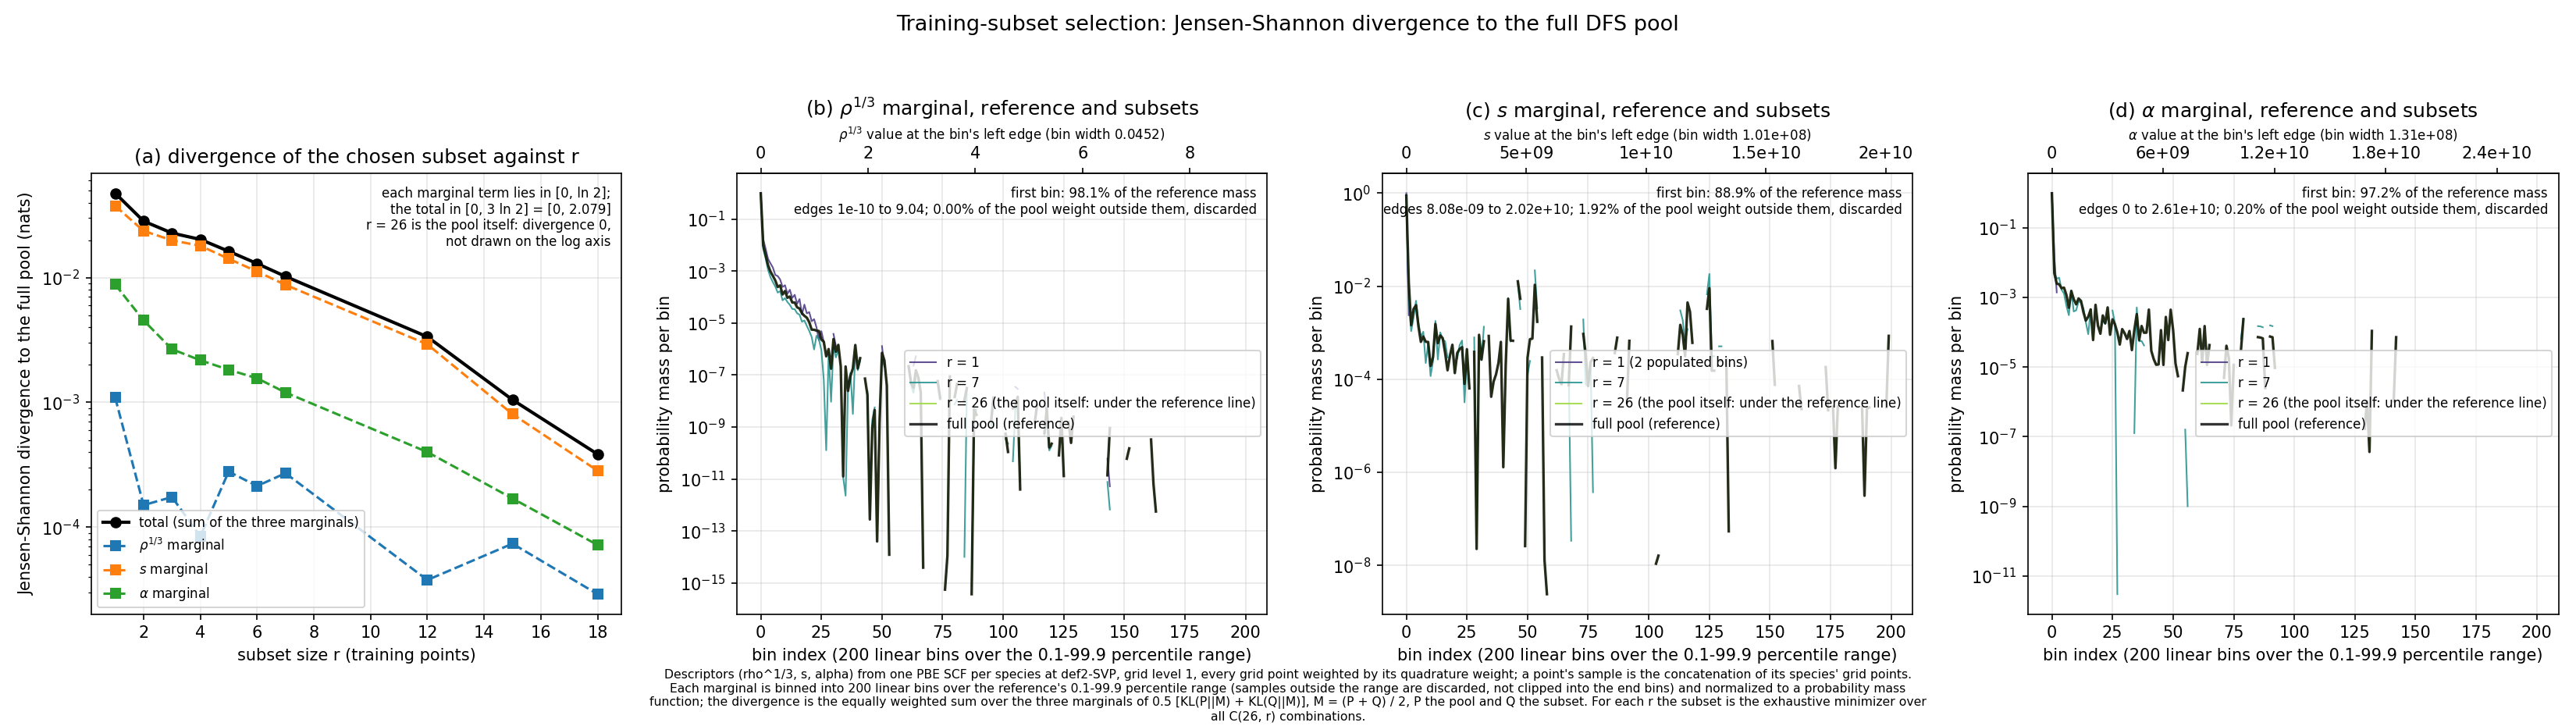
\includegraphics[width=\linewidth,height=0.9\textheight,keepaspectratio]{figures_dfs_step7_v7_subsets/subset_jsd_vs_full.png}\end{center}
\end{landscape}


\section*{3. Pre-training (functional cloning)}

Sources: \path{xcquinox/alec/pretrain.py}, \path{xcquinox/alec/pretrain_data_gen.py}, the \path{pretrain:} and \path{fidelity:} blocks of the resolved configurations, \path{pretrain/<arch>/pretrain_metadata.json} and \path{pretrain/<arch>/fidelity_certificate.json} of each run.

\subsection*{3.1 Set, targets and objective}

Each network is fitted to reproduce its parent functional's enhancement factor pointwise on the parent's own self-consistent densities: PBE for the GGA rung, SCAN for the meta-GGA rung. The set is the DFS pre-training inventory (8 free atoms and 22 G2/97 molecules at the GGA level; 20 molecules at the meta-GGA level, which drops H2 and N2) plus every single-atom species of the BH76 and W4-11 pools at its production charge and spin (the 12 neutral elements and the F- and Cl- anions), 39 systems for the GGA groups and 38 for the meta-GGA group (\path{n_systems} of the certificates). The targets are stored per grid point as

\[
t_x = F_x^{\rm parent} - 1 = \frac{\epsilon_x^{\rm parent}}{\epsilon_x^{\rm LDA}} - 1, \qquad
t_c = F_c^{\rm parent} - 1 = \frac{\epsilon_c^{\rm parent}}{\epsilon_c^{\rm PW92}} - 1,
\]

from spin-resolved libxc evaluations, the exchange rows posed per spin channel at the doubled density $(2 n_\sigma, 4\sigma_{\sigma\sigma})$, the footing the production exchange evaluates (\texttt{exchange\_footing: spin\_channel}). A synthetic $(r_s, s, \alpha)$ mesh (the DFS SI's $(s, \alpha)$ grid extended to three dimensions) is added as a regularizer at a fixed 30 percent share of the integration weight (\texttt{mesh\_fraction: 0.3}); its rows belong to no system.

The objective per network is the integration-weighted pointwise residual plus a per-system energy term (\path{_PretrainLoss}):

\[
\begin{aligned}
\mathcal{L}_{\rm pre} = {} & \frac{\sum_i w_i\,(F_i^{\rm NN} - 1 - t_i)^2}{\sum_i w_i} \\
& + w_E\,\frac{1}{N_{\rm sys}}\sum_{s}\Big(\sum_{i\in s} w^{\rm grid}_i\, n_i\,\epsilon_i^{\rm LDA}\, F_i^{\rm NN} - E_{xc,s}^{\rm parent}\Big)^2,
\end{aligned}
\]

\[
w_i = |n_i\, \epsilon_i^{\rm LDA}|\, w_i^{\rm grid}, \qquad w_E = 0.1 .
\]

The energy term is present because the pointwise residual alone does not bound a system's energy: in the earlier campaign the architecture with the lowest exchange residual carried the largest atomization-energy offset from its parent. Schedule: Adam, 20000 steps, learning rate $10^{-3}$ decaying linearly to $10^{-5}$ from the midpoint, gradient clip 1.0, a 20 percent held-out validation slice scored every 50 steps with patience 300 checks (\path{pretrain:} block).

\subsection*{3.2 The fidelity certificate}

After the fit, the saved networks are re-evaluated on every system of the set at the production basis and grid and compared with the parent: the per-system exchange-correlation energy error $\Delta E_{xc,s} = E_{xc,s}^{\rm NN} - E_{xc,s}^{\rm parent}$, and, for every molecule, the atomization-energy error $\Delta AE = \Delta E_{xc,{\rm mol}} - \sum_A \Delta E_{xc,A}$ against the parent's own atomization energy. The gate (\path{fidelity:} block, two-tier since 2026-09-02) is

\[
\max_{\rm atoms} |\Delta E_{xc,A}| \le 1.0\ \text{mHa}, \qquad
\mathrm{mean}_{\rm mol} |\Delta AE| \le 1.0\ \text{kcal/mol}, \qquad
\max_{\rm mol} |\Delta AE| \le 2.0\ \text{kcal/mol},
\]

and a failing certificate makes the pre-training task exit without success, which holds the group's preflight and training array. The certificate is what gives the training-stage comparison against PBE (or SCAN) its meaning: every trained cell starts from a network that is its parent to within these tolerances.

\subsection*{3.3 Pre-training loss curves}

\textbf{Fig. 3.1} The pointwise term of the objective per step taken, for the exchange network (left) and the correlation network (right), one curve per architecture, log scale over the 20000 steps; the final value of each curve is printed in the legend. The regular spikes from step 5000 onward are the validation checks: every 50 steps the objective is evaluated on the held-out slice and the best network is snapshotted, and the training step that follows a snapshot reload sits above the trend line for one step. The first figure holds the seven certified GGA clones of the size and families runs; the second the meta-GGA clone (its certificate failed, so it is not in the merged view and is drawn from its run).

The exchange curves of the two Glorot-start architectures reach $6.4 \times 10^{-8}$ (deep\_3x16) and $1.5 \times 10^{-8}$ (deep\_attn\_3x16), the correlation curves $7.6 \times 10^{-7}$ and $6.7 \times 10^{-8}$; deep\_attn\_3x16 descends earliest and ends lowest on both networks. Of the zero-init architectures deep0\_attn\_3x16 is lowest on both networks ($1.5 \times 10^{-8}$, $1.0 \times 10^{-7}$), deep0\_3x16 and deep0\_cusp\_3x16 within a factor 3.5 of each other ($2.8 \times 10^{-8}$ and $9.5 \times 10^{-8}$; $3.4 \times 10^{-6}$ and $1.1 \times 10^{-6}$). The meta-GGA clone stops at $3.7 \times 10^{-6}$ (exchange) and $5.2 \times 10^{-6}$ (correlation), 40 to 250 times above the GGA clones in exchange and 1.5 to 80 times in correlation after the same 20000 steps, with a smooth trajectory and no divergence.

\begin{landscape}
\begin{center}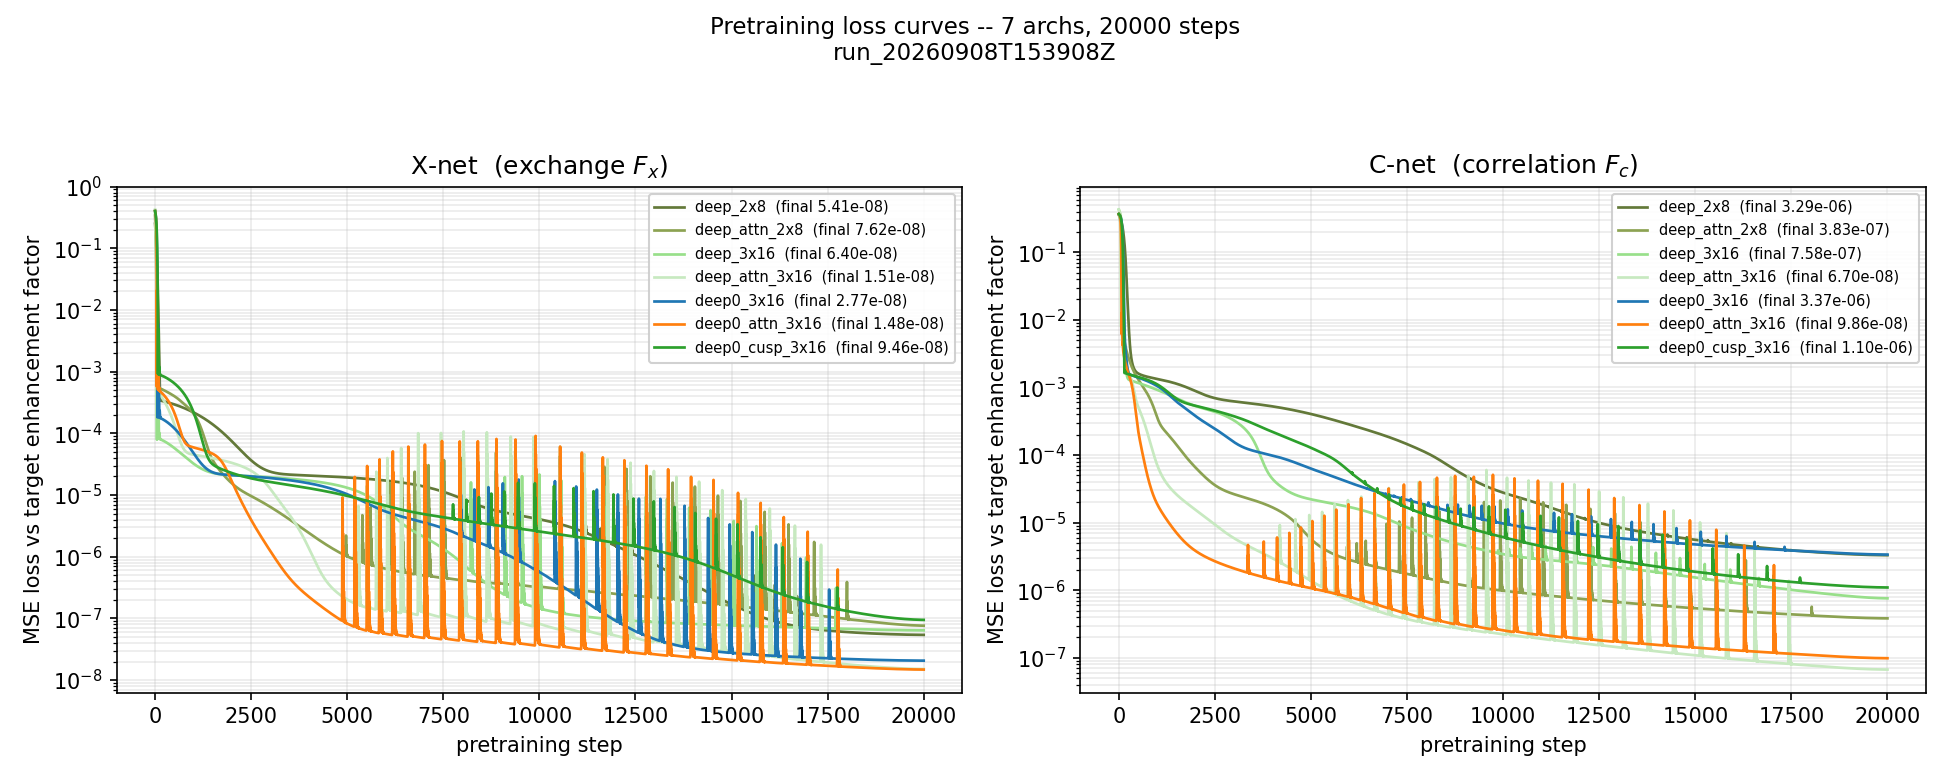
\includegraphics[width=\linewidth,height=0.9\textheight,keepaspectratio]{figures_dfs_step7_v7_family_pretrain/pretrain_curves.png}\end{center}
\begin{center}
\includegraphics[width=\linewidth,height=0.9\textheight,keepaspectratio]{figures_dfs_step7_v7_family_pretrain/uncertified_mgga/pretrain_curves.png}\end{center}
\end{landscape}


\subsection*{3.4 Certificate summary}

\textbf{Fig. 3.2} One bar per architecture, the mean $|\Delta AE|$ against the parent over the set's molecules; the marker above each bar is the largest single-species $|\Delta AE|$, with the species above 1 kcal/mol printed beside it. Blue bars are the v7 round (this campaign, the two-tier gate: the dashed line at 1.0 kcal/mol gates the mean, the dotted line at 2.0 kcal/mol every species), one colour per run (the size run, the families run, the meta-GGA run); the meta-GGA bar is the FAILED certificate, hatched, with its flagged species printed. The numbers are in the table of Sec. 3.6. Reading: every v7 bar sits below 0.35 kcal/mol and every v7 marker below 1.5 kcal/mol; the attention architectures are the tightest (deep\_attn\_3x16 0.031 mean, 0.115 max; deep0\_attn\_3x16 0.042 and 0.149), deep0\_cusp\_3x16 the loosest (0.188 mean, 1.071 max on AlCl3).

\begin{landscape}
\begin{center}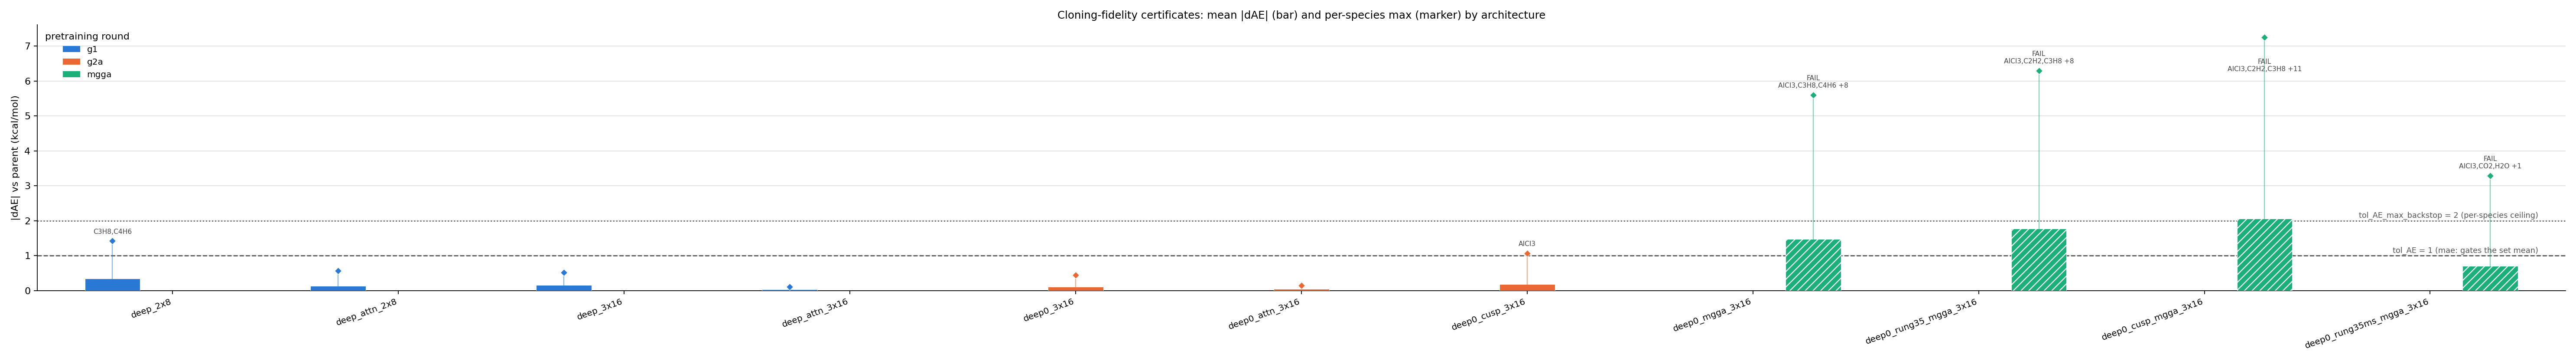
\includegraphics[width=\linewidth,height=0.9\textheight,keepaspectratio]{figures_dfs_step7_v7_family_pretrain/certificate_summary.png}\end{center}
\end{landscape}


\subsection*{3.5 Pre-trained enhancement factors}

\textbf{Fig. 3.3} For one architecture, the pre-trained network against its parent along two slices of descriptor space. Top left: the exchange enhancement factor $F_x(s)$ at density $n = 1$ and zero extra descriptors, the parent dashed, the network solid, from $s = 0$ to 6. Top right: the difference $F_x^{\rm NN} - F_x^{\rm parent}$ on the same slice, which is where the fit is visible at all. Bottom left: the correlation factor $F_c(s; r_s)$ at $\zeta = 0$ for $r_s = 0.5$, 2 and 5, parent dashed and network solid; bottom right: the three differences. For the meta-GGA clone the layout is three columns: $F_x(s; \alpha)$ at $\alpha = 0$ and $\alpha = 1$ (the SCAN Fig. 1 convention, $\alpha$ the exact iso-orbital indicator of the slice) and $F_c$ at the same two $\alpha$ values, each with its difference panel. The footer of each figure names the run, the slices, the largest $|\Delta F_x|$ on the slice and the certificate verdict.

deep\_3x16: $|\Delta F_x| \le 7 \times 10^{-3}$ over $s \le 6$, a smooth negative deviation growing beyond $s = 4$ (the region the pre-training set barely samples), $|\Delta F_c| \le 4.5 \times 10^{-3}$ with oscillations below $s = 1.5$ at every $r_s$. deep\_attn\_3x16: $|\Delta F_x| \le 6 \times 10^{-3}$, $|\Delta F_c| \le 10^{-2}$ with one dip at $s = 2$, $r_s = 0.5$. deep0\_3x16: $|\Delta F_x| \le 2.6 \times 10^{-3}$ (the tightest exchange clone of the three shown), $|\Delta F_c| \le 1.2 \times 10^{-2}$ at $r_s = 0.5$ and 5. deep0\_cusp\_mgga\_3x16 against SCAN: $F_x$ at $\alpha = 0$ runs 0.005 below SCAN up to $s = 1$ and 0.01 to 0.027 above it for $s > 2.5$ (the maximum at $s = 4.3$), and $F_x$ at $\alpha = 1$ 0.005 to 0.013 below it between $s = 1$ and 4; $F_c$ at $\alpha = 1$, $r_s = 0.5$ has a spike of $+0.04$ near $s = 0.2$, a dip of $-0.022$ at $s = 0.8$ and sits 0.005 to 0.033 below SCAN from $s = 2$ onward; at $\alpha = 0$ the correlation differences stay within $\pm 0.02$. These are systematic, same-sign offsets over wide ranges of $s$, which is the shape of error that does not cancel between a molecule and its atoms (Sec. 3.6).

\begin{center}
\includegraphics[width=\linewidth,height=0.92\textheight,keepaspectratio]{figures_dfs_step7_v7_family_pretrain/pretrain_fx_fc_deep_3x16.png}\end{center}
\begin{center}
\includegraphics[width=\linewidth,height=0.92\textheight,keepaspectratio]{figures_dfs_step7_v7_family_pretrain/pretrain_fx_fc_deep_attn_3x16.png}\end{center}
\begin{center}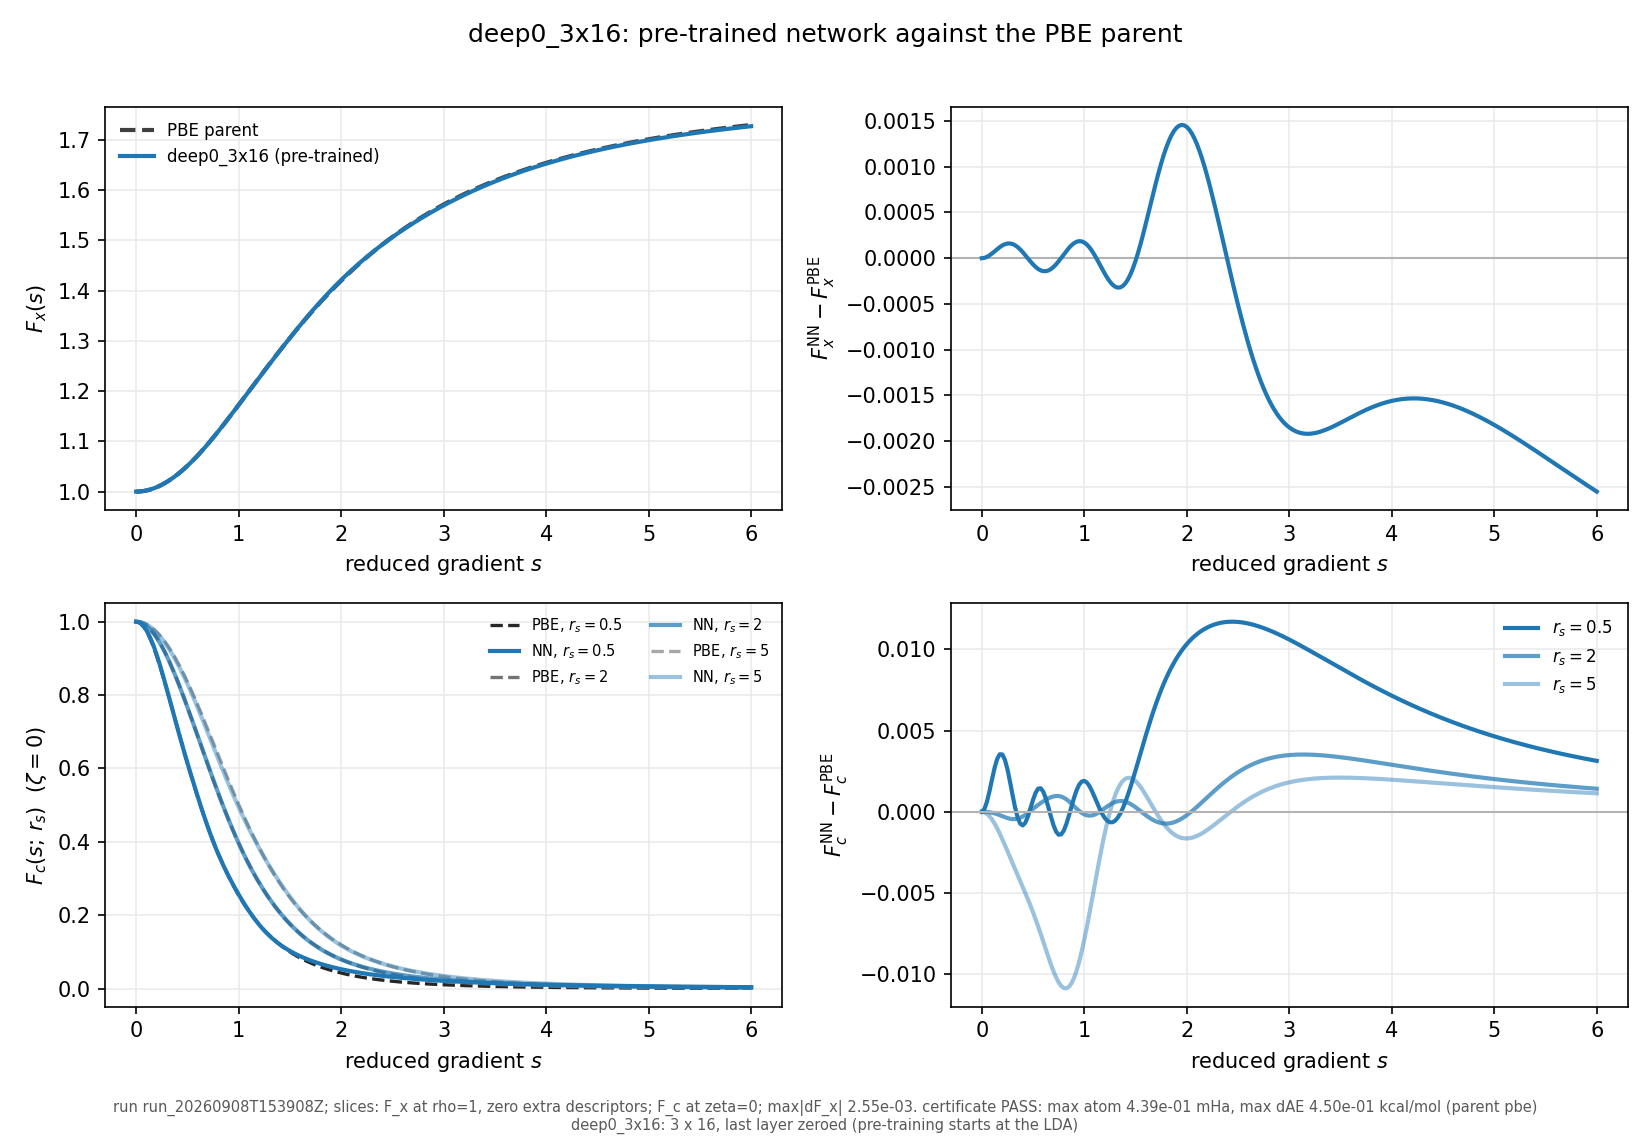
\includegraphics[width=\linewidth,height=0.92\textheight,keepaspectratio]{figures_dfs_step7_v7_family_pretrain/pretrain_fx_fc_deep0_3x16.png}\end{center}
\begin{center}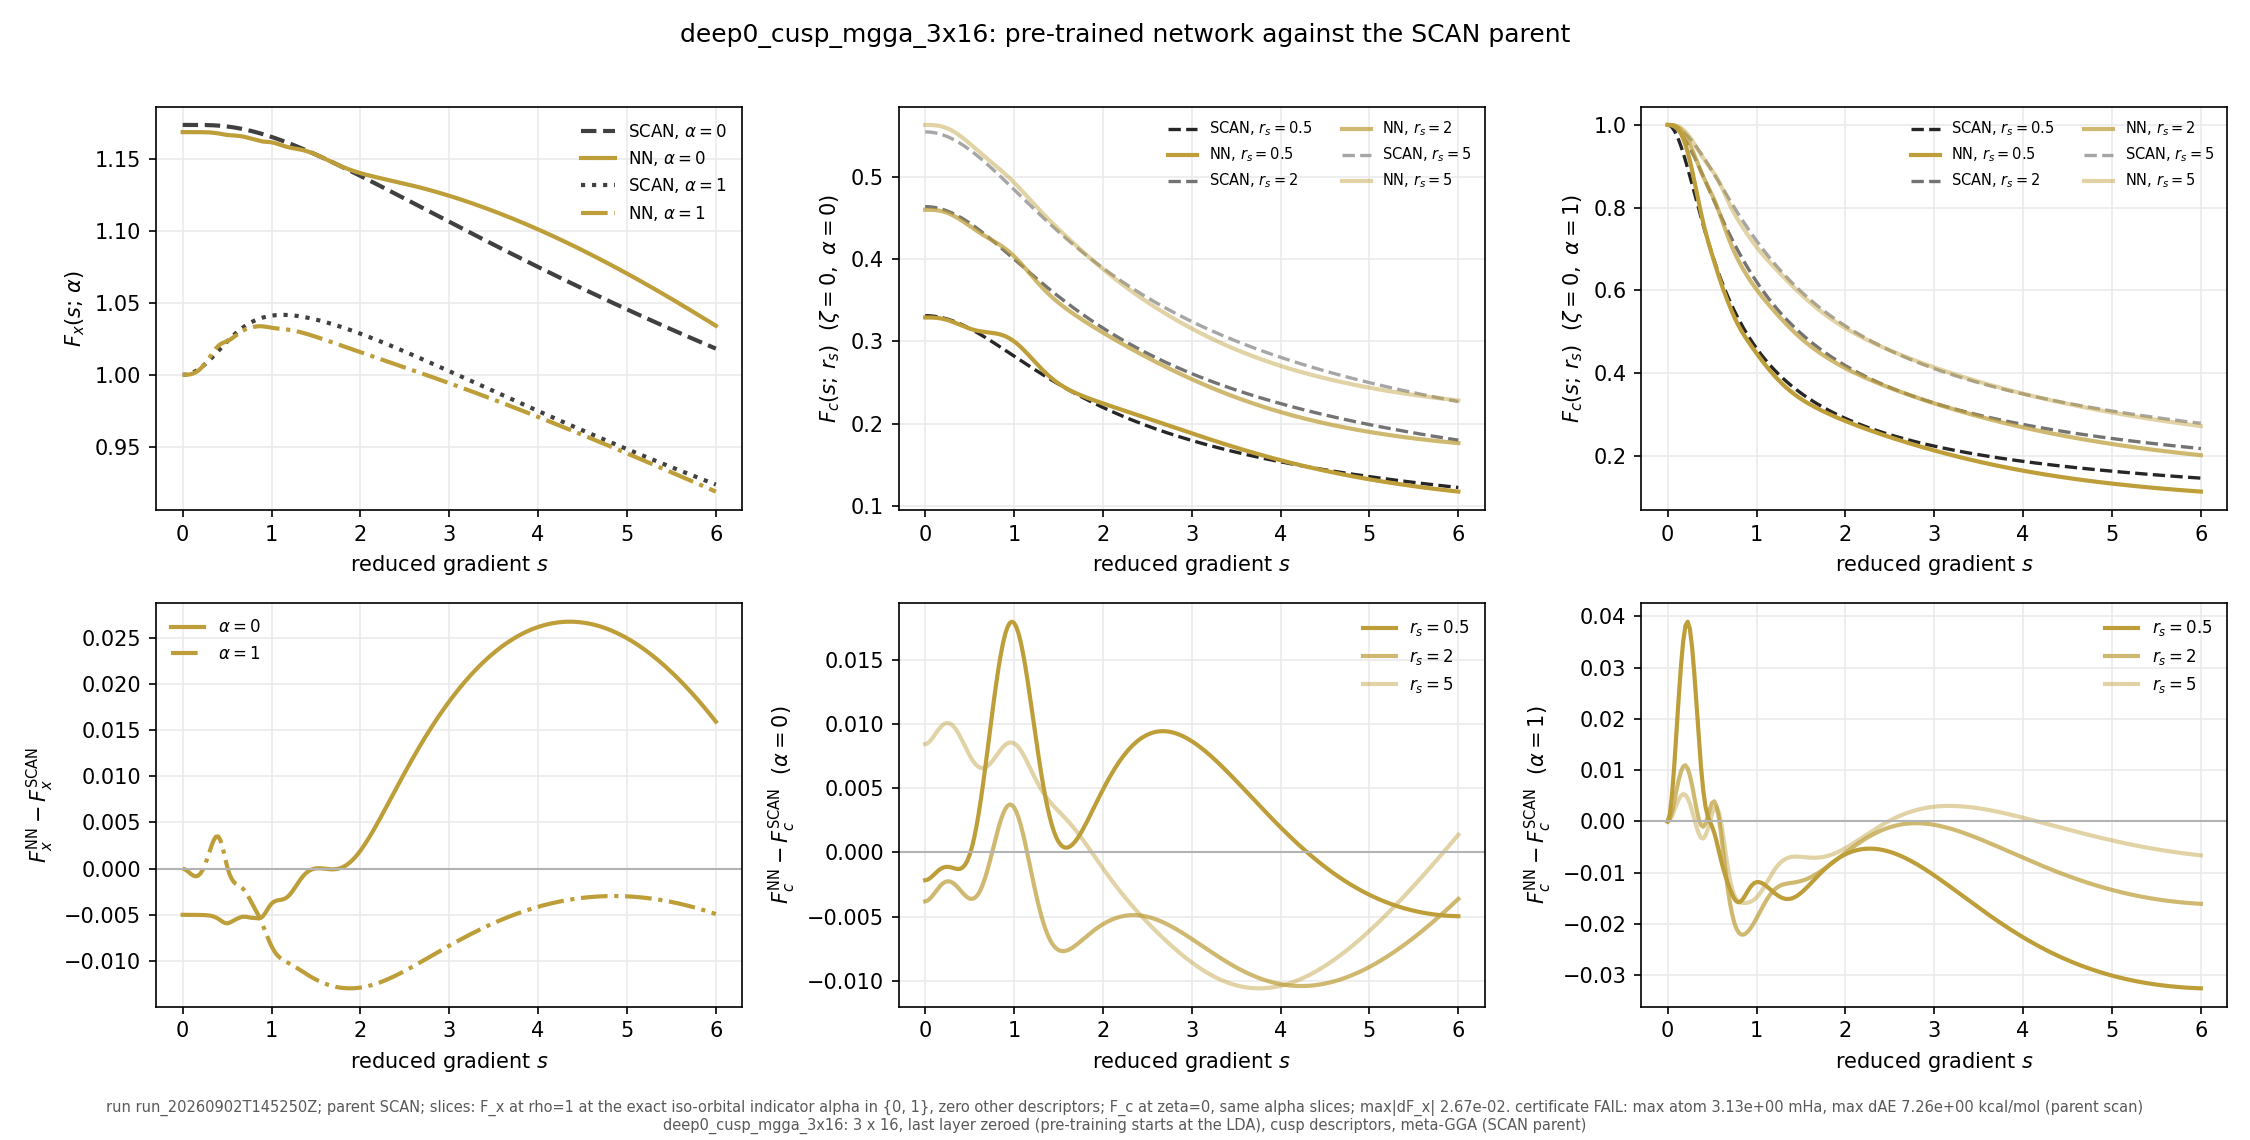
\includegraphics[width=\linewidth,height=0.92\textheight,keepaspectratio]{figures_dfs_step7_v7_family_pretrain/uncertified_mgga/pretrain_fx_fc_deep0_cusp_mgga_3x16.png}\end{center}


\textbf{Fig. 3.4} The exchange differences (left) and the correlation differences at $r_s = 2$ (right) of every certified GGA clone on one pair of axes. The two Glorot-start exchange clones agree with PBE to $1 \times 10^{-3}$ below $s = 2.5$ and fan out beyond it (deep\_attn\_3x16 to $+0.003$ at $s = 3.9$, and at $s = 6$ deep\_3x16 $-0.007$, deep\_attn\_3x16 $-0.006$); their correlation clones stay within $3 \times 10^{-3}$ below $s = 3$, deep\_attn\_3x16 drifting to $+5 \times 10^{-3}$ by $s = 6$. The three zero-init clones stay within $4.2 \times 10^{-3}$ everywhere on both slices (deep0\_attn\_3x16 exchange $+0.0034$ at $s = 4.2$; deep0\_cusp\_3x16 correlation $+0.0041$ at $s = 3.2$).

\begin{landscape}
\begin{center}
\includegraphics[width=\linewidth,height=0.9\textheight,keepaspectratio]{figures_dfs_step7_v7_family_pretrain/pretrain_fx_fc_delta_all.png}\end{center}
\end{landscape}


The deep0\_attn\_3x16 and deep0\_cusp\_3x16 clones are drawn in the same directories (\path{pretrain_fx_fc_<arch>.png}).

\subsection*{3.6 Certificate results}

Read from \path{pretrain/<arch>/fidelity_certificate.json} and \path{pretrain_metadata.json}; the pointwise losses are the saved network's, in units of the squared enhancement-factor residual.

Every GGA clone passes on all three criteria; the one with a species above 1 kcal/mol (deep0\_cusp\_3x16: AlCl3) passes on the mean and under the 2.0 kcal/mol backstop. The attention variants are the tightest clones by every measure (deep\_attn\_3x16: max atom 0.058 mHa, mean 0.031 kcal/mol; deep0\_attn\_3x16: 0.123 mHa, 0.042 kcal/mol), at the price of the longest fits (about 28 h against 3.6 to 3.8 h for their plain twins, \path{duration_seconds}).

The meta-GGA clone deep0\_cusp\_mgga\_3x16 fails all three criteria after a converged 20000-step fit (pointwise residuals 3.7e-6 and 5.2e-6, an order of magnitude above the GGA clones'): the largest free-atom error is 3.13 mHa (O; B 2.91, Be 2.61), the mean atomization error 2.06 kcal/mol and the largest 7.26 kcal/mol (C4H6; C3H8 7.19, O2 4.77, SiCH6 3.52, CH4 3.47), 14 of 22 molecules above 1 kcal/mol, every one of the eight largest errors of the same sign. Fig. 3.3 (bottom) shows where the clone misses SCAN: the $\alpha = 0$ exchange slice is 0.015 to 0.027 above SCAN for $s > 2$ and the $\alpha = 1$ correlation slices sit 0.01 to 0.03 below it at $r_s = 0.5$, systematic offsets that do not cancel between a molecule and its atoms. The v6 meta-GGA certificates, all PASS, were fitted in the anchored model class (the network learns a correction on top of SCAN); this is the first unanchored meta-GGA clone the two-tier gate has judged. The four remaining meta-GGA architectures are pending; whether the rung or this architecture is the cause is decided by their certificates. Until then the meta-GGA training array is held.

\begin{landscape}
\begin{scriptsize}
\begin{longtable}{lllllp{0.116\linewidth}p{0.116\linewidth}p{0.116\linewidth}p{0.116\linewidth}l}
\toprule Run & Architecture & Parent & Steps & Pointwise loss X / C & max atom $\lvert\Delta E_{xc}\rvert$ (mHa) & mean $\lvert\Delta AE\rvert$ (kcal/mol) & max $\lvert\Delta AE\rvert$ (kcal/mol) & Species over 1 kcal/mol & Verdict \\ \midrule \endhead
size & deep\_3x16 & PBE & 20000 & 6.40e-08 / 7.58e-07 & 0.210 & 0.162 & 0.519 & none & PASS \\
size & deep\_attn\_3x16 & PBE & 20000 & 1.51e-08 / 6.70e-08 & 0.058 & 0.031 & 0.115 & none & PASS \\
families & deep0\_3x16 & PBE & 20000 & 2.77e-08 / 3.37e-06 & 0.439 & 0.114 & 0.450 & none & PASS \\
families & deep0\_attn\_3x16 & PBE & 20000 & 1.48e-08 / 9.86e-08 & 0.123 & 0.042 & 0.149 & none & PASS \\
families & deep0\_cusp\_3x16 & PBE & 20000 & 9.46e-08 / 1.10e-06 & 0.439 & 0.188 & 1.071 & AlCl3 & PASS \\
meta-GGA & deep0\_cusp\_mgga\_3x16 & SCAN & 20000 & 3.70e-06 / 5.18e-06 & 3.132 & 2.062 & 7.257 & AlCl3, C2H2, C3H8, C4H6, CH2, CH4, CO, CO2, F2, H2O, HCN, O2, PH3, SiCH6 & FAIL \\
\bottomrule \end{longtable}
\end{scriptsize}
\end{landscape}


\section*{4. Optimization, in-sample}

Sources: \path{xcquinox/alec/losses.py} (\path{L5_gradnorm_vxc_step7}, the channel terms), \path{xcquinox/alec/train.py} (the per-molecule loop, the optimizer), \path{xcquinox/alec/oneshot.py} (the SCF tail window), \path{xcquinox/alec/solver_manual.py} (the differentiable SCF), the \path{hyperparams:} and \path{solvers:} blocks of the resolved configurations, and per cell \path{train_metadata.json}, \path{losses.npy}, \path{aux_log.pkl}, \path{eval/per_molecule.json}.

\subsection*{4.1 Training protocol}

Each cell trains the certified clone of its architecture on a subset of the 26-point DFS pool. The per-molecule update scheme takes one optimizer step per training group (a reaction, or a molecule with its density and potential references) per epoch, so an epoch is one pass over the groups. The loss of a group is the fixed weighted sum

\[
\mathcal{L} = 1\cdot\mathcal{L}_{AE} + 1\cdot\mathcal{L}_{\rm rxn} + 1\cdot\mathcal{L}_{IP} + 1\cdot\mathcal{L}_{v_{xc}} + 20\cdot\mathcal{L}_{\rho},
\]

the Letter's $\lambda_{RE} = 1$, $\lambda_n = 20$ structure (\path{effective_channel_weights}; the GradNorm balancer is configured but dormant under this scheme, and the \path{vxc_weight} 0.01 and \path{density_weight} 0.1 pre-scales are forced to 1). The channels, with $E^{\rm NN}$ the self-consistent total energy of the 3-cycle SCF (Sec. 4.2) and $t = 0, \ldots, N-1$ the cycle index:

\begin{itemize}
\item Reaction energies (\texttt{ae\_as\_reactions: true} routes the W4-11 atomizations here as molecule-to-atoms reactions with the network's own atoms, beside the BH76 barriers): \[
\mathcal{L}_{\rm rxn} = \frac{1}{|T|}\sum_{t\in T} w_t^2\, r_t^2, \qquad
r_t = \sum_i c_i\, E^{\rm NN}_{i,t} - E^{\rm ref}, \qquad
w_t = \left(\frac{t}{N-1}\right)^2,
\] $T$ the kept SCF tail (the last $\min(N, 10)$ cycles; at $N = 3$ all three, $w_t^2 = 0, 1/16, 1$), the DFS convergence-tail scoring (DFS Eqs. 15 and 16) that penalizes a non-converging SCF instead of one arbitrary final cycle. Absolute Ha$^2$ (\texttt{loss\_metric: absolute}). References: W4-11 atomization energies and the W2-F12 BH76 barrier heights of GMTKN55.
\item Atom anchors (the residue of the AE channel once the atomizations are reactions): the free atoms of the subset are held near their exact non-relativistic energies $E_Z^{\rm anchor}$ (Chakravorty et al., PRA 47, 3649 (1993)), $\mathcal{L}_{AE} = 0.01\cdot\mathrm{mean}_Z\, (E_Z^{\rm NN} - E_Z^{\rm anchor})^2 / (E_Z^{\rm anchor})^2$.
\item Ionization potentials, $\mathcal{L}_{IP} = \mathrm{mean}\,(E^{\rm NN}_{+} - E^{\rm NN}_0 - IP^{\rm ref})^2$, present in the form but empty on every v7 subset (no IP13 point is selected).
\item Exchange-correlation potential, on the reference density (frozen features): $\mathcal{L}_{v_{xc}} = \|V_{xc}^{\rm NN} - V_{xc}^{\rm ref}\|_F^2 / n_{\rm AO}^2$, summed over spin channels for open shells.
\item Density, the final mixed density of the SCF against the CCSD reference density on the same grid, per electron squared (the Letter's Eq. 17 normalization; \texttt{density\_per\_electron: true}): \[
\mathcal{L}_{\rho} = \mathrm{mean}_{\rm mol}\,\frac{\sum_g w_g\,(n^{\rm NN}_g - n^{\rm ref}_g)^2}{N_e^2},
\qquad N_e = \sum_g w_g\, n^{\rm ref}_g .
\]
\end{itemize}

Optimizer: AdamW, learning rate $10^{-3}$ held for the first half of the run and decayed linearly to $10^{-5}$ over the second (\texttt{lr\_decay\_start: 0.5}), weight decay $10^{-4}$, gradient clip 1.0. 200 epochs (\path{n_steps}), a validation reaction-energy MAE on the 35-reaction validation slice every 25 epochs, early stop after 5 checks without a 0.1 kcal/mol improvement; three checkpoints are kept (final, lowest training loss, lowest validation MAE), and the figures of Secs. 4 and 5 read the validation-best one. Over the 33 cells the runs took 150 to 200 epochs (early-stopped in 17) and 1.2 to 34.9 h of wall each (\path{train_metadata.json}).

\subsection*{4.2 The differentiable SCF}

The energies and densities above are self-consistent: the manual backend runs a fixed $N = 3$ cycles from the converged PBE density (\texttt{solver: full\_3}), diagonalizing the Kohn-Sham matrix built from the network's $V_{xc}$ each cycle, with the DFS decaying linear mixing $D_{t+1} = (1 - a_t) D_t + a_t D^{\rm out}_t$, $a_t = 0.3^{t} + 0.3$, a freeze once $|\Delta E| < 10^{-6}$ Ha, and gradients through every cycle. The density scored by $\mathcal{L}_\rho$ and by the density metrics is the last mixed density; three cycles do not converge the SCF for a functional far from a fixed point, which is the subject of the two arms submitted on 2026-09-08 (25 cycles; dpyscf parity) and of the converged-SCF re-evaluation in flight. The density record of 2026-09-07 (\path{notebooks/analysis/AUDIT_2026-09-01.md}, the density section) records the full parity table against dpyscf.

\subsection*{4.3 Training losses}

\textbf{Fig. 4.1} Per-channel training losses, one figure per architecture, eight panels. Every loss panel is the weighted per-epoch mean over the epoch's group updates read from the cell's \path{aux_log.pkl}, on a log axis against the epoch, one curve per subset size (the color bar: dark one molecule, yellow twenty-six). Panel 1 is the total loss, the quantity the optimizer steps; panels 2 to 6 are the five channels of Sec. 4.1 at their trained weights, and they add up to panel 1 at every epoch. Panel 7 is the validation reaction-energy MAE at each 25-epoch check, the star marking the validation-best epoch whose checkpoint every later figure reads. The footer states the weights and their source.

deep\_3x16 (the first figure): the total falls from 1.3e-4 to 2.1e-4 at the first epoch to a plateau reached by epoch 25 in every cell, the plateau ordered by subset size from 3.7e-5 (one molecule) to 1.0e-4 (eighteen), because the potential and density channels grow with the number of supervised molecules. The reaction channel is the one that falls by orders of magnitude: from 1e-4 at the first epoch to 4e-9 (one molecule), 2e-6 to 8e-6 (two to six) and 1.6e-5 to 3.1e-5 (seven to twenty-six) at the end. The anchors channel is 1e-8 to 1e-6 throughout and drifts upward in the large-subset cells (the free atoms are released as the molecules pull the functional). The ionization channel (present from three molecules, where Li+ enters the subset) peaks at 1e-5 within the first 50 epochs and falls to 1e-6 to 4e-6. The potential channel is the one that rises: from 1e-5 to 1.3e-5 at the start to 1.4e-5 (one to six molecules) and 2.4e-5 to 4.3e-5 (seven to twenty-six) at the end, the rise steepest in the first 25 epochs. The density channel drops from 2.6e-5 to 4.8e-5 to 1.0e-5 (one molecule) and 1.8e-5 to 2.5e-5 (the rest) inside the first 10 epochs and is flat afterwards. The validation panel separates the cells into two families: the two-to-six-molecule cells start at 12 to 19 kcal/mol and rise to 15 to 33 by the last check (the star at epoch 25 for two, three, five and six; at 200 for four, whose MAE falls back from 20 to 14.6), while the one-molecule cell and the cells from seven upward hold 7 to 10 kcal/mol across every check.

deep\_attn\_3x16 (the second figure): the same shapes with a reaction channel that falls further (5e-7 to 2e-6 at two to six molecules, 8e-7 at seven), a density channel that ends lower (6e-6 to 1.3e-5), and a validation panel where the two-to-six-molecule cells fall rather than rise: from 22 to 37 kcal/mol at the first check to 7 to 13 by epoch 100, with the validation-best epochs at 75 to 200. deep0\_3x16 (the third figure) reproduces the deep\_3x16 picture, validation included (two molecules: 11.2 to 32.4 kcal/mol; seven to eighteen: 6.2 to 8.8).

The first and last five-epoch means of every channel and every validation check are in the table of Sec. 4.5.

\begin{landscape}
\begin{center}
\includegraphics[width=\linewidth,height=0.9\textheight,keepaspectratio]{figures_dfs_step7_v7_family_val_best/training_loss_channels_deep_3x16.png}\end{center}
\begin{center}
\includegraphics[width=\linewidth,height=0.9\textheight,keepaspectratio]{figures_dfs_step7_v7_family_val_best/training_loss_channels_deep_attn_3x16.png}\end{center}
\begin{center}
\includegraphics[width=\linewidth,height=0.9\textheight,keepaspectratio]{figures_dfs_step7_v7_family_val_best/training_loss_channels_deep0_3x16.png}\end{center}
\end{landscape}


\textbf{Fig. 4.2} The total training loss per cell as a rolling mean over the group updates (log axis against the fraction of the run's updates; the first panel of Fig. 4.1 on the update rather than the epoch axis), one panel per architecture, one curve per subset size. The curves are the quantity stepped; the fall between the first and the last five percent of the updates is the "loss fall" column of the table in Sec. 4.5 (1.2 to 5.1 over the 33 cells). The deep\_3x16 panel separates into the two plateaus of Fig. 4.1 (1e-4 for the cells from twelve molecules upward, 3e-5 to 5e-5 below); the one-molecule curve alternates between two levels from update to update. The deep\_attn\_3x16 panel shows transient rises near 45 and 70 percent of the run in the one- and two-molecule cells, the spikes of the potential and density channels around epochs 85 to 105 in Fig. 4.1.

\begin{center}
\includegraphics[width=\linewidth,height=0.92\textheight,keepaspectratio]{figures_dfs_step7_v7_family_val_best/training_loss_total.png}\end{center}


\subsection*{4.4 Trained enhancement factors}

\textbf{Fig. 4.3} The trained networks against PBE, one figure per architecture, four panels, one curve per subset size at the validation-best checkpoint. Top left: $F_x(s)$ at $n = 1$ and zero extra descriptors, PBE dashed. Top right: $F_x^{\rm NN} - F_x^{\rm PBE}$ on the same slice. Bottom left: $F_c(s; r_s = 2)$ at $\zeta = 0$, PBE dashed. Bottom right: the correlation difference. The pre-trained curves of Fig. 3.3 are the starting point of every curve here, and the footer gives the largest $|\Delta F_x|$ over the slice.

Exchange, all three architectures: every trained network lowers $F_x$ below PBE between $s = 0.3$ and 1.3 (by 0.02 to 0.06 at $s \approx 0.8$) and raises it above PBE from $s \approx 1.4$ onward, with the maximum of the raise at $s = 2.5$ to 3 (deep\_3x16 up to 0.18; deep\_attn\_3x16 0.07 to 0.13; deep0\_3x16 0.05 to 0.14) and a slow decay to $+0.03$ to $+0.06$ at $s = 6$, so that the trained $F_x$ crosses 1.7 near $s = 3.5$ where PBE crosses it near $s = 5$. The shape is the same at every subset size; the one-molecule cell moves least. Correlation at $r_s = 2$: PBE's $F_c$ falls from 1 at $s = 0$ to 0.02 at $s = 3$; every trained network holds $F_c$ between 0.6 and 1.0 up to $s = 2$, and beyond that the cells separate. deep\_3x16: the one-molecule cell returns to PBE (a difference of 0.2 at $s = 1$ and 0 beyond 3), the two- and three-molecule cells rise to 1.1 to 1.4 at $s = 6$, the four-to-six-molecule cells decay to 0.15 to 0.25 and the cells from seven to twenty-six molecules to 0.4 to 0.6. deep0\_3x16: the one-molecule cell as for deep\_3x16, the two-molecule cell 1.5 at $s = 6$, the fifteen-molecule cell flat at 0.8 from $s = 2$, the twelve- and eighteen-molecule cells 1.1 to 1.2, the others 0.1 to 0.25. deep\_attn\_3x16: the one-molecule cell returns to PBE, every other cell rises above 1 from $s = 2$ to 3 onward, to 1.2 (two molecules), 1.4 (three and seven), 1.7 (four) and 1.9 (five and six) at $s = 6$. The correlation difference therefore reaches 0.2 to 1.9 at large $s$ depending on the cell. The corrections are therefore not small perturbations of PBE: the density-gradient dependence of both channels is reshaped in the region $s > 1.5$, which is populated by the valence tails and the bonding regions of molecules, and what Sec. 5 measures is how that reshaping transfers.

\begin{center}
\includegraphics[width=\linewidth,height=0.92\textheight,keepaspectratio]{figures_dfs_step7_v7_family_val_best/trained_fx_fc_deep_3x16.png}\end{center}
\begin{center}
\includegraphics[width=\linewidth,height=0.92\textheight,keepaspectratio]{figures_dfs_step7_v7_family_val_best/trained_fx_fc_deep_attn_3x16.png}\end{center}
\begin{center}
\includegraphics[width=\linewidth,height=0.92\textheight,keepaspectratio]{figures_dfs_step7_v7_family_val_best/trained_fx_fc_deep0_3x16.png}\end{center}


\subsection*{4.5 In-sample fit}

\textbf{Fig. 4.4} Training-set density against CCSD in grid-RMSE units, final checkpoint (the in-sample evaluation exists for the final checkpoint only; its validation-best twin is identical because the in-sample directory is shared). Left: the cell mean over the trained species against the subset size (the species count printed at each point), one line per architecture, with PBE on the same species as the dashed line with crosses. Middle: every trained species on the abscissa (22, the union of the subsets, the same for every run), the network's RMSE at every cell that trained it as a point and PBE's as a cross, log scale: the network's points sit below the cross for most species, FLi and HLi (0.7e-5 to 2e-5 against 1.5e-5 and 4e-5) and the second-row hydrides among them, and above it for a few (C2H2 in the small-subset cells). Right: the NN/PBE ratio of the cell means against the subset size, PBE at 1: deep\_3x16 0.72 at one molecule, 0.81 to 0.97 at two to six, 0.73 to 0.79 from seven; deep\_attn\_3x16 0.57 to 0.76; deep0\_3x16 0.68 to 0.93; deep0\_attn\_3x16 0.64 and 0.91 at one and two molecules. The table below gives the ratios and the count of improved species per cell (198 of the 233 (cell, species) pairs over the 33 cells, 50 of deep\_attn\_3x16's 51).

\begin{landscape}
\begin{center}
\includegraphics[width=\linewidth,height=0.9\textheight,keepaspectratio]{figures_dfs_step7_v7_family_val_best/insample_density_vs_ccsd.png}\end{center}
\end{landscape}


\textbf{Fig. 4.5} In-sample energy and density in DFS units, the 3x3 layout of Fig. 5.5 on the training set: rows WTMAD-2 / $\varepsilon_n$ / $\mathcal{ED}$, columns BH76 / W4-11 / combined, each cell against PBE on its own training reactions and molecules. The energy leg is the training reactions themselves (the W4-11 atomizations as molecule-to-atoms reactions and the BH76 barriers of \path{train_metadata.json}), each formed from the final checkpoint's self-consistent species energies in \path{eval/per_molecule.json} against its reference; PBE on the same reactions from the same file's PBE energies. The dashed line is PBE on the union of the run's training reactions (18.6 kcal/mol for the BH76 barriers, 3.83 for the W4-11 atomizations, 5.67 combined, the same union for every run since the runs train the same subsets); the capped spans and the verdict triangles use each cell's own reactions. A cell whose subset has no reaction of a column (the one-molecule cell in the BH76 column; the three-molecule cell, whose subset is H2O, Li+ and a barrier, in the W4-11 column) has no bar there.

Panel A (BH76 energy): deep\_3x16's barrier residual grows with the subset from 2.7 kcal/mol at two molecules to 9.5 at twenty-six, against 18.6 for PBE on the union and 12 to 25 on the cells' own barriers; deep\_attn\_3x16 0.8 to 3.2. Panel B (W4-11): deep\_3x16 0.02 (one molecule, H2O fitted to 0.02 kcal/mol) to 1.6, deep\_attn\_3x16 0.05 to 0.36, against PBE's 3.83. Panel C: the two-subset combination, 0.02 to 4.3 against 5.67 on the union of the training reactions of every cell. Panels D to F (density): the trained molecules' $\varepsilon_n$ is 0.0073 (one molecule) to 0.0135 (two) for deep\_3x16 and 0.0049 to 0.0073 for deep\_attn\_3x16, against PBE's 0.0089 on the union of the trained molecules; the deep\_3x16 cells at two to seven molecules sit above PBE on this per-electron L1 while their grid RMSE (Fig. 4.4) sits below it: the two norms rank the small-subset fits differently. Panels G to I: every cell's $\mathcal{ED}$ is below PBE's on its own slice (0.002 to 8.5 against 0.8 to 13.3), the energy leg deciding the combination at every subset.

\begin{landscape}
\begin{center}
\includegraphics[width=\linewidth,height=0.9\textheight,keepaspectratio]{figures_dfs_step7_v7_family_val_best/insample_by_pool_3x3_eps.png}\end{center}
\end{landscape}


\subsection*{4.6 Results per cell}

The training-set density panels (Fig. 4.4) are the direct check that the density channel trains: on the supervised molecules the cell-mean density RMSE against CCSD is below PBE's in all 33 cells, the NN/PBE ratio 0.72 to 0.97 for deep\_3x16, 0.57 to 0.76 for deep\_attn\_3x16, 0.68 to 0.93 for deep0\_3x16 and 0.64 and 0.91 for deep0\_attn\_3x16 at one and two molecules, with the weakest fits at two to six molecules and 198 of the 233 trained species-cells improved (the second table below, computed from \path{eval/per_molecule.json} with case twins collapsed). The total loss (Fig. 4.2) falls by a factor 1.2 to 5.1 between the first and the last 5 percent of the updates and is flat by the end.

Per channel (Fig. 4.1; the first table below gives the first and last five-epoch means of every weighted channel, computed from the logs, and the third the validation checks): the reaction channel falls in every cell, by 3x (deep0\_3x16 at 18 molecules) to 190x (deep\_attn\_3x16 at 2), and the density channel by 1.3x to 4.6x, both settling within the first 25 epochs; the potential channel, the term the DFS objective does not carry (Sec. 4.2), rises over training from seven to eighteen molecules in the deep\_3x16 and deep0\_3x16 cells (deep\_3x16 at 12: 2.2e-5 to 2.8e-5; at 18: 3.9e-5 to 4.3e-5), is flat at 26 (3.7e-5 in both) and falls in the attention cells at 12 and 15 (deep\_attn\_3x16: 2.6e-5 to 2.5e-5, 3.3e-5 to 2.9e-5); the anchors channel stays at 1e-7 to 1e-6 and the ionization channel (populated from three molecules, where the Li ionization enters) peaks in the first 50 epochs and falls. The validation MAE of the 2-to-6-molecule cells of deep\_3x16 and deep0\_3x16 rises after the first check (deep\_3x16 at 2: 11.7 to 32.7 kcal/mol, validation-best at epoch 25), while the same cells of deep\_attn\_3x16 fall over the run, and deep0\_attn\_3x16 splits (at 1: 7.8 to 15.1, best at 25; at 2: 33.8 to 23.7, best at 150); the cells from seven molecules upward hold 6 to 11 kcal/mol across their checks (deep\_attn\_3x16 at 12 opens at 11.0 and ends at 8.0; deep\_3x16 at 26 peaks at 10.4). The held-out rise at the same subset sizes is recorded in Sec. 5.8.

\begin{landscape}
\textbf{Training losses per cell} (\path{aux_log.pkl} of each cell; the weighted per-epoch means of the first and last five epochs; the channel weights 1, 1, 1, 1, 20 of Sec. 4.1).

\begin{scriptsize}
\begin{longtable}{llllllllll}
\toprule Run & Architecture & Subset & Epochs & total first/last & AE first/last & reactions first/last & IP13 first/last & V\_xc first/last & rho first/last \\ \midrule \endhead
size & deep\_3x16 & 1 & 175 & 4.47e-5 / 3.66e-5 & 7.77e-8 / 1.93e-7 & 7.25e-7 / 4.16e-9 & 0.00e+0 / 0.00e+0 & 3.13e-5 / 2.68e-5 & 1.26e-5 / 9.62e-6 \\
size & deep\_3x16 & 2 & 150 & 1.79e-4 / 4.29e-5 & 1.66e-7 / 7.16e-7 & 1.31e-4 / 4.49e-6 & 0.00e+0 / 0.00e+0 & 1.35e-5 / 1.73e-5 & 3.43e-5 / 2.05e-5 \\
size & deep\_3x16 & 3 & 150 & 1.83e-4 / 3.85e-5 & 4.91e-8 / 7.93e-8 & 1.36e-4 / 2.04e-6 & 5.12e-6 / 2.63e-6 & 1.39e-5 / 1.37e-5 & 2.82e-5 / 2.01e-5 \\
size & deep\_3x16 & 4 & 200 & 1.57e-4 / 4.19e-5 & 4.50e-8 / 3.98e-8 & 1.10e-4 / 3.05e-6 & 3.94e-6 / 2.06e-6 & 1.21e-5 / 1.33e-5 & 3.12e-5 / 2.35e-5 \\
size & deep\_3x16 & 5 & 150 & 1.39e-4 / 4.10e-5 & 3.75e-8 / 6.83e-8 & 9.16e-5 / 5.96e-6 & 1.08e-5 / 2.89e-6 & 1.07e-5 / 1.25e-5 & 2.62e-5 / 1.96e-5 \\
size & deep\_3x16 & 6 & 150 & 1.34e-4 / 4.51e-5 & 2.52e-8 / 7.90e-8 & 8.98e-5 / 8.13e-6 & 7.05e-6 / 2.11e-6 & 1.01e-5 / 1.33e-5 & 2.70e-5 / 2.15e-5 \\
size & deep\_3x16 & 7 & 200 & 1.58e-4 / 5.90e-5 & 1.29e-7 / 2.96e-8 & 9.01e-5 / 1.60e-5 & 8.12e-6 / 1.89e-6 & 1.69e-5 / 2.35e-5 & 4.29e-5 / 1.76e-5 \\
size & deep\_3x16 & 12 & 200 & 2.14e-4 / 8.38e-5 & 1.03e-7 / 4.38e-8 & 1.40e-4 / 3.07e-5 & 4.65e-6 / 1.56e-6 & 2.17e-5 / 2.79e-5 & 4.78e-5 / 2.36e-5 \\
size & deep\_3x16 & 15 & 150 & 1.96e-4 / 8.79e-5 & 1.03e-7 / 8.94e-8 & 1.15e-4 / 3.02e-5 & 4.00e-6 / 1.50e-6 & 2.92e-5 / 3.39e-5 & 4.74e-5 / 2.22e-5 \\
size & deep\_3x16 & 18 & 150 & 1.94e-4 / 1.03e-4 & 1.05e-7 / 2.08e-7 & 1.08e-4 / 3.13e-5 & 3.45e-6 / 3.78e-6 & 3.92e-5 / 4.31e-5 & 4.38e-5 / 2.46e-5 \\
size & deep\_3x16 & 26 & 175 & 1.79e-4 / 9.16e-5 & 1.98e-7 / 1.84e-7 & 9.34e-5 / 2.76e-5 & 3.08e-6 / 1.15e-6 & 3.73e-5 / 3.73e-5 & 4.54e-5 / 2.53e-5 \\
size & deep\_attn\_3x16 & 1 & 150 & 4.49e-5 / 2.28e-5 & 1.48e-7 / 7.30e-7 & 3.63e-7 / 1.39e-8 & 0.00e+0 / 0.00e+0 & 3.49e-5 / 1.60e-5 & 9.52e-6 / 6.03e-6 \\
size & deep\_attn\_3x16 & 2 & 200 & 1.44e-4 / 2.11e-5 & 3.02e-7 / 2.63e-7 & 9.54e-5 / 5.08e-7 & 0.00e+0 / 0.00e+0 & 1.36e-5 / 1.29e-5 & 3.43e-5 / 7.44e-6 \\
size & deep\_attn\_3x16 & 3 & 200 & 1.51e-4 / 2.30e-5 & 8.53e-8 / 2.28e-7 & 9.82e-5 / 6.22e-7 & 7.06e-6 / 3.99e-8 & 1.32e-5 / 1.37e-5 & 3.28e-5 / 8.41e-6 \\
size & deep\_attn\_3x16 & 4 & 200 & 1.25e-4 / 2.40e-5 & 4.86e-8 / 3.67e-8 & 8.16e-5 / 1.36e-6 & 4.99e-6 / 1.87e-8 & 1.16e-5 / 1.26e-5 & 2.66e-5 / 9.94e-6 \\
size & deep\_attn\_3x16 & 5 & 200 & 1.12e-4 / 2.00e-5 & 7.20e-8 / 7.07e-8 & 6.49e-5 / 1.49e-6 & 1.12e-5 / 4.01e-8 & 1.06e-5 / 1.09e-5 & 2.51e-5 / 7.51e-6 \\
size & deep\_attn\_3x16 & 6 & 200 & 1.04e-4 / 2.27e-5 & 4.82e-8 / 3.52e-8 & 6.12e-5 / 2.06e-6 & 6.95e-6 / 1.19e-7 & 1.05e-5 / 1.15e-5 & 2.57e-5 / 8.98e-6 \\
size & deep\_attn\_3x16 & 7 & 200 & 1.18e-4 / 3.43e-5 & 1.18e-7 / 1.77e-7 & 5.79e-5 / 8.12e-7 & 7.39e-6 / 4.76e-7 & 1.98e-5 / 1.98e-5 & 3.24e-5 / 1.30e-5 \\
size & deep\_attn\_3x16 & 12 & 200 & 1.64e-4 / 6.37e-5 & 1.05e-7 / 3.10e-7 & 9.69e-5 / 1.72e-5 & 4.93e-6 / 1.39e-6 & 2.63e-5 / 2.51e-5 & 3.61e-5 / 1.97e-5 \\
size & deep\_attn\_3x16 & 15 & 200 & 1.43e-4 / 6.59e-5 & 1.56e-7 / 6.95e-7 & 7.06e-5 / 1.80e-5 & 5.18e-6 / 1.02e-6 & 3.26e-5 / 2.94e-5 & 3.43e-5 / 1.67e-5 \\
families & deep0\_3x16 & 1 & 175 & 4.46e-5 / 3.20e-5 & 5.86e-8 / 4.65e-8 & 8.47e-7 / 3.81e-10 & 0.00e+0 / 0.00e+0 & 3.12e-5 / 2.33e-5 & 1.25e-5 / 8.61e-6 \\
families & deep0\_3x16 & 2 & 150 & 1.80e-4 / 3.69e-5 & 1.37e-7 / 8.33e-7 & 1.35e-4 / 1.59e-6 & 0.00e+0 / 0.00e+0 & 1.33e-5 / 1.59e-5 & 3.09e-5 / 1.86e-5 \\
families & deep0\_3x16 & 3 & 150 & 1.82e-4 / 4.23e-5 & 3.82e-8 / 8.71e-8 & 1.37e-4 / 3.21e-6 & 4.91e-6 / 7.03e-6 & 1.35e-5 / 1.36e-5 & 2.60e-5 / 1.83e-5 \\
families & deep0\_3x16 & 4 & 200 & 1.55e-4 / 3.96e-5 & 4.02e-8 / 3.46e-8 & 1.10e-4 / 3.40e-6 & 3.92e-6 / 4.92e-6 & 1.18e-5 / 1.25e-5 & 2.93e-5 / 1.87e-5 \\
families & deep0\_3x16 & 5 & 150 & 1.38e-4 / 3.91e-5 & 3.06e-8 / 3.63e-8 & 9.35e-5 / 5.75e-6 & 1.00e-5 / 4.56e-6 & 1.04e-5 / 1.15e-5 & 2.42e-5 / 1.72e-5 \\
families & deep0\_3x16 & 6 & 150 & 1.33e-4 / 4.26e-5 & 2.23e-8 / 5.93e-8 & 9.04e-5 / 7.17e-6 & 6.70e-6 / 3.65e-6 & 9.91e-6 / 1.25e-5 & 2.57e-5 / 1.92e-5 \\
families & deep0\_3x16 & 7 & 200 & 1.53e-4 / 4.92e-5 & 1.42e-7 / 1.90e-8 & 8.72e-5 / 8.77e-6 & 8.61e-6 / 3.00e-6 & 1.71e-5 / 2.09e-5 & 4.03e-5 / 1.65e-5 \\
families & deep0\_3x16 & 12 & 200 & 2.11e-4 / 7.79e-5 & 1.22e-7 / 1.17e-8 & 1.36e-4 / 2.77e-5 & 4.97e-6 / 1.66e-6 & 2.21e-5 / 2.72e-5 & 4.71e-5 / 2.13e-5 \\
families & deep0\_3x16 & 15 & 200 & 1.93e-4 / 8.08e-5 & 1.30e-7 / 2.62e-8 & 1.13e-4 / 2.78e-5 & 4.52e-6 / 1.62e-6 & 2.93e-5 / 3.18e-5 & 4.60e-5 / 1.97e-5 \\
families & deep0\_3x16 & 18 & 150 & 1.86e-4 / 9.83e-5 & 1.42e-7 / 1.21e-7 & 1.01e-4 / 3.13e-5 & 4.22e-6 / 2.23e-6 & 3.84e-5 / 4.10e-5 & 4.26e-5 / 2.36e-5 \\
families & deep0\_3x16 & 26 & 150 & 1.76e-4 / 8.92e-5 & 2.06e-7 / 1.50e-7 & 9.07e-5 / 2.71e-5 & 3.24e-6 / 1.35e-6 & 3.76e-5 / 3.74e-5 & 4.47e-5 / 2.33e-5 \\
families & deep0\_attn\_3x16 & 1 & 150 & 4.48e-5 / 2.50e-5 & 1.32e-7 / 8.15e-7 & 3.07e-7 / 1.30e-8 & 0.00e+0 / 0.00e+0 & 3.48e-5 / 1.67e-5 & 9.49e-6 / 7.50e-6 \\
families & deep0\_attn\_3x16 & 2 & 200 & 1.52e-4 / 3.29e-5 & 2.43e-7 / 2.68e-7 & 1.04e-4 / 6.97e-7 & 0.00e+0 / 0.00e+0 & 1.33e-5 / 1.49e-5 & 3.51e-5 / 1.70e-5 \\
\bottomrule \end{longtable}
\end{scriptsize}
\end{landscape}


\begin{landscape}
\textbf{Validation checks per cell} (the validation reaction-energy MAE at every 25-epoch check and the epoch whose checkpoint the figures read).

\begin{footnotesize}
\begin{longtable}{llllp{0.493\linewidth}l}
\toprule Run & Architecture & Subset & Epochs & Validation MAE at each 25-epoch check (kcal/mol) & Validation-best epoch \\ \midrule \endhead
size & deep\_3x16 & 1 & 175 & 9.4, 8.2, 8.4, 9.1, 9.0, 9.1, 9.1 & 50 \\
size & deep\_3x16 & 2 & 150 & 11.7, 25.2, 28.1, 30.0, 31.3, 32.7 & 25 \\
size & deep\_3x16 & 3 & 150 & 14.6, 22.5, 22.0, 17.0, 16.0, 15.6 & 25 \\
size & deep\_3x16 & 4 & 200 & 18.2, 20.0, 16.6, 15.6, 15.4, 14.9, 14.7, 14.6 & 200 \\
size & deep\_3x16 & 5 & 150 & 19.2, 23.4, 23.3, 26.8, 27.6, 27.7 & 25 \\
size & deep\_3x16 & 6 & 150 & 18.4, 21.1, 21.9, 22.6, 22.2, 22.4 & 25 \\
size & deep\_3x16 & 7 & 200 & 7.8, 7.3, 7.4, 7.1, 6.9, 7.2, 6.9, 7.0 & 175 \\
size & deep\_3x16 & 12 & 200 & 9.0, 8.5, 8.3, 8.7, 8.1, 7.8, 7.9, 7.9 & 150 \\
size & deep\_3x16 & 15 & 150 & 7.3, 8.0, 7.6, 7.5, 7.9, 7.5 & 25 \\
size & deep\_3x16 & 18 & 150 & 7.1, 8.0, 7.3, 8.0, 7.2, 7.3 & 25 \\
size & deep\_3x16 & 26 & 175 & 9.3, 8.9, 9.3, 9.0, 10.4, 9.3, 9.7 & 50 \\
size & deep\_attn\_3x16 & 1 & 150 & 8.2, 13.8, 17.9, 18.7, 15.8, 17.0 & 25 \\
size & deep\_attn\_3x16 & 2 & 200 & 36.5, 31.3, 24.0, 16.9, 9.6, 7.6, 7.2, 7.2 & 200 \\
size & deep\_attn\_3x16 & 3 & 200 & 29.5, 21.7, 13.3, 15.6, 17.8, 19.4, 20.8, 21.2 & 75 \\
size & deep\_attn\_3x16 & 4 & 200 & 22.1, 12.7, 7.4, 7.3, 8.0, 7.8, 7.6, 8.1 & 100 \\
size & deep\_attn\_3x16 & 5 & 200 & 25.0, 15.4, 9.8, 9.8, 12.1, 12.7, 13.3, 13.4 & 100 \\
size & deep\_attn\_3x16 & 6 & 200 & 22.4, 19.5, 10.6, 9.9, 8.9, 8.6, 8.9, 9.0 & 150 \\
size & deep\_attn\_3x16 & 7 & 200 & 7.2, 5.9, 5.9, 5.7, 6.6, 6.5, 6.7, 6.7 & 100 \\
size & deep\_attn\_3x16 & 12 & 200 & 11.0, 9.0, 8.1, 9.2, 8.1, 7.2, 8.0, 8.0 & 150 \\
size & deep\_attn\_3x16 & 15 & 200 & 7.2, 8.0, 8.1, 8.4, 6.3, 6.8, 7.0, 7.3 & 125 \\
families & deep0\_3x16 & 1 & 175 & 10.3, 9.3, 9.4, 10.0, 10.4, 11.8, 12.5 & 50 \\
families & deep0\_3x16 & 2 & 150 & 11.2, 26.0, 31.1, 31.8, 32.0, 32.4 & 25 \\
families & deep0\_3x16 & 3 & 150 & 14.0, 22.9, 22.0, 20.2, 18.6, 17.1 & 25 \\
families & deep0\_3x16 & 4 & 200 & 15.4, 16.7, 14.9, 13.0, 12.4, 11.9, 11.8, 11.7 & 200 \\
families & deep0\_3x16 & 5 & 150 & 13.1, 22.1, 21.4, 22.6, 23.3, 23.4 & 25 \\
families & deep0\_3x16 & 6 & 150 & 13.5, 17.3, 17.0, 17.4, 17.3, 17.8 & 25 \\
families & deep0\_3x16 & 7 & 200 & 8.1, 6.8, 6.7, 6.4, 6.2, 6.7, 6.4, 6.5 & 125 \\
families & deep0\_3x16 & 12 & 200 & 9.2, 8.1, 8.1, 8.5, 7.7, 7.8, 8.0, 8.0 & 125 \\
families & deep0\_3x16 & 15 & 200 & 7.6, 8.0, 7.5, 7.5, 8.4, 8.3, 8.6, 8.8 & 75 \\
families & deep0\_3x16 & 18 & 150 & 7.6, 8.3, 7.7, 8.7, 8.2, 8.4 & 25 \\
families & deep0\_3x16 & 26 & 150 & 8.9, 9.0, 8.9, 8.8, 9.7, 9.2 & 100 \\
families & deep0\_attn\_3x16 & 1 & 150 & 7.8, 9.2, 9.5, 9.6, 10.3, 15.1 & 25 \\
families & deep0\_attn\_3x16 & 2 & 200 & 33.8, 29.2, 26.6, 26.6, 27.1, 23.7, 25.5, 26.0 & 150 \\
\bottomrule \end{longtable}
\end{footnotesize}
\end{landscape}


On the training reactions themselves (Fig. 4.5, the table below): every one of the 33 cells is below PBE on the DFS-units $\mathcal{ED}$ over its own training reactions and molecules; the training-reaction WTMAD-2 is 0.00 to 4.4 kcal/mol against 5.7 for PBE on the union of the training reactions, the attention twins the closest fits (deep\_attn\_3x16 0.05 to 2.45, deep0\_attn\_3x16 0.05 and 0.77). The training-molecule $\varepsilon_n$ sits above PBE's pooled value in every deep\_3x16 cell but 1 and 26 and every deep0\_3x16 cell but 1, 18 and 26, below it in every deep\_attn\_3x16 cell and in deep0\_attn\_3x16 at 1 (above at 2), while the grid RMSE of the same molecules is below PBE's in every cell: the per-electron L1 and the grid RMSE rank the same fits differently, and both are reported.

\textbf{In-sample per cell in DFS units} (\path{insample_by_pool_3x3_eps.csv} of the family \path{_val_best} set, identical in the final-step set; combined leg; E = 2-subset WTMAD-2 over the cell's own training reactions, kcal/mol; eps over its training molecules; ED under gamma = 1084.87 kcal/mol; the PBE columns are the union of the run's training reactions / molecules for E and eps and the cell's own slice for ED; n = training reactions and trained species with a density).

\begin{landscape}
\begin{footnotesize}
\begin{longtable}{llllllllllll}
\toprule Architecture & Subset & n rxn & n species & E NN & E PBE (pool) & eps NN & eps PBE (pool) & ED NN & ED PBE (cell) & dED & beats \\ \midrule \endhead
deep\_3x16 & 1 & 1 & 1 & 0.02 & 5.67 & 0.00728 & 0.00888 & 0.05 & 0.79 & \textbf{-0.74} & yes \\
deep\_3x16 & 2 & 2 & 3 & 2.14 & 5.67 & 0.01353 & 0.00888 & 3.73 & 11.27 & \textbf{-7.55} & yes \\
deep\_3x16 & 3 & 2 & 3 & 2.96 & 5.67 & 0.01106 & 0.00888 & 4.75 & 12.57 & \textbf{-7.82} & yes \\
deep\_3x16 & 4 & 3 & 4 & 2.63 & 5.67 & 0.01118 & 0.00888 & 4.33 & 11.58 & \textbf{-7.25} & yes \\
deep\_3x16 & 5 & 3 & 4 & 4.31 & 5.67 & 0.01315 & 0.00888 & 6.63 & 13.25 & \textbf{-6.63} & yes \\
deep\_3x16 & 6 & 4 & 5 & 3.92 & 5.67 & 0.01234 & 0.00888 & 6.06 & 11.78 & \textbf{-5.72} & yes \\
deep\_3x16 & 7 & 5 & 6 & 2.04 & 5.67 & 0.01042 & 0.00888 & 3.46 & 7.89 & \textbf{-4.44} & yes \\
deep\_3x16 & 12 & 10 & 11 & 3.11 & 5.67 & 0.01026 & 0.00888 & 4.86 & 8.86 & \textbf{-4.00} & yes \\
deep\_3x16 & 15 & 13 & 14 & 2.78 & 5.67 & 0.00900 & 0.00888 & 4.32 & 8.08 & \textbf{-3.76} & yes \\
deep\_3x16 & 18 & 16 & 16 & 2.60 & 5.67 & 0.00944 & 0.00888 & 4.14 & 8.01 & \textbf{-3.86} & yes \\
deep\_3x16 & 26 & 24 & 22 & 2.23 & 5.67 & 0.00731 & 0.00888 & 3.49 & 7.14 & \textbf{-3.66} & yes \\
deep\_attn\_3x16 & 1 & 1 & 1 & 0.05 & 5.67 & 0.00494 & 0.00888 & 0.09 & 0.79 & \textbf{-0.70} & yes \\
deep\_attn\_3x16 & 2 & 2 & 3 & 0.59 & 5.67 & 0.00617 & 0.00888 & 1.08 & 11.27 & \textbf{-10.20} & yes \\
deep\_attn\_3x16 & 3 & 2 & 3 & 1.57 & 5.67 & 0.00626 & 0.00888 & 2.55 & 12.57 & \textbf{-10.02} & yes \\
deep\_attn\_3x16 & 4 & 3 & 4 & 1.68 & 5.67 & 0.00648 & 0.00888 & 2.71 & 11.58 & \textbf{-8.87} & yes \\
deep\_attn\_3x16 & 5 & 3 & 4 & 1.77 & 5.67 & 0.00732 & 0.00888 & 2.89 & 13.25 & \textbf{-10.36} & yes \\
deep\_attn\_3x16 & 6 & 4 & 5 & 1.72 & 5.67 & 0.00724 & 0.00888 & 2.83 & 11.78 & \textbf{-8.96} & yes \\
deep\_attn\_3x16 & 7 & 5 & 6 & 0.53 & 5.67 & 0.00640 & 0.00888 & 0.98 & 7.89 & \textbf{-6.92} & yes \\
deep\_attn\_3x16 & 12 & 10 & 11 & 2.45 & 5.67 & 0.00784 & 0.00888 & 3.80 & 8.86 & \textbf{-5.05} & yes \\
deep\_attn\_3x16 & 15 & 13 & 14 & 2.20 & 5.67 & 0.00667 & 0.00888 & 3.37 & 8.08 & \textbf{-4.70} & yes \\
deep0\_3x16 & 1 & 1 & 1 & 0.00 & 5.67 & 0.00753 & 0.00888 & 0.00 & 0.79 & \textbf{-0.79} & yes \\
deep0\_3x16 & 2 & 2 & 3 & 0.91 & 5.67 & 0.01392 & 0.00888 & 1.72 & 11.27 & \textbf{-9.56} & yes \\
deep0\_3x16 & 3 & 2 & 3 & 3.81 & 5.67 & 0.01046 & 0.00888 & 5.71 & 12.57 & \textbf{-6.86} & yes \\
deep0\_3x16 & 4 & 3 & 4 & 2.92 & 5.67 & 0.00969 & 0.00888 & 4.57 & 11.58 & \textbf{-7.01} & yes \\
deep0\_3x16 & 5 & 3 & 4 & 4.36 & 5.67 & 0.01327 & 0.00888 & 6.69 & 13.25 & \textbf{-6.56} & yes \\
deep0\_3x16 & 6 & 4 & 5 & 3.61 & 5.67 & 0.01257 & 0.00888 & 5.71 & 11.78 & \textbf{-6.08} & yes \\
deep0\_3x16 & 7 & 5 & 6 & 1.58 & 5.67 & 0.01038 & 0.00888 & 2.77 & 7.89 & \textbf{-5.12} & yes \\
deep0\_3x16 & 12 & 10 & 11 & 3.00 & 5.67 & 0.01037 & 0.00888 & 4.74 & 8.86 & \textbf{-4.12} & yes \\
deep0\_3x16 & 15 & 13 & 14 & 2.72 & 5.67 & 0.00913 & 0.00888 & 4.27 & 8.08 & \textbf{-3.80} & yes \\
deep0\_3x16 & 18 & 16 & 16 & 2.66 & 5.67 & 0.00873 & 0.00888 & 4.16 & 8.01 & \textbf{-3.85} & yes \\
deep0\_3x16 & 26 & 24 & 22 & 2.22 & 5.67 & 0.00721 & 0.00888 & 3.46 & 7.14 & \textbf{-3.68} & yes \\
deep0\_attn\_3x16 & 1 & 1 & 1 & 0.05 & 5.67 & 0.00508 & 0.00888 & 0.09 & 0.79 & \textbf{-0.70} & yes \\
deep0\_attn\_3x16 & 2 & 2 & 3 & 0.77 & 5.67 & 0.01118 & 0.00888 & 1.45 & 11.27 & \textbf{-9.83} & yes \\
\bottomrule \end{longtable}
\end{footnotesize}
\end{landscape}


\begin{landscape}
\textbf{In-sample density fit per cell} (\path{eval/per_molecule.json}; the cell mean of the grid RMSE against CCSD over the trained species, twins collapsed; the loss fall is the ratio of the mean total loss over the first five percent of the updates to that over the last five percent).

\begin{scriptsize}
\begin{longtable}{llllllllll}
\toprule Run & Architecture & Subset & Trained species & Density RMSE NN & PBE & NN/PBE & Species improved & Loss fall (first/last 5\%) & Updates \\ \midrule \endhead
size & deep\_3x16 & 1 & 1 & 9.52e-05 & 1.32e-04 & 0.72 & 1/1 & 1.2 & 525 \\
size & deep\_3x16 & 2 & 3 & 8.28e-05 & 1.03e-04 & 0.81 & 2/3 & 3.7 & 600 \\
size & deep\_3x16 & 3 & 3 & 1.29e-04 & 1.33e-04 & 0.97 & 2/3 & 4.4 & 750 \\
size & deep\_3x16 & 4 & 4 & 1.16e-04 & 1.22e-04 & 0.96 & 2/4 & 3.4 & 1200 \\
size & deep\_3x16 & 5 & 4 & 9.34e-05 & 1.03e-04 & 0.90 & 2/4 & 3.5 & 1050 \\
size & deep\_3x16 & 6 & 5 & 8.99e-05 & 1.02e-04 & 0.88 & 3/5 & 2.7 & 1200 \\
size & deep\_3x16 & 7 & 6 & 1.03e-04 & 1.32e-04 & 0.78 & 5/6 & 2.2 & 1800 \\
size & deep\_3x16 & 12 & 11 & 1.17e-04 & 1.49e-04 & 0.79 & 8/11 & 2.0 & 2800 \\
size & deep\_3x16 & 15 & 14 & 1.10e-04 & 1.45e-04 & 0.76 & 11/14 & 1.9 & 2550 \\
size & deep\_3x16 & 18 & 16 & 1.21e-04 & 1.52e-04 & 0.79 & 13/16 & 1.6 & 3000 \\
size & deep\_3x16 & 26 & 22 & 1.18e-04 & 1.60e-04 & 0.73 & 20/22 & 1.6 & 4900 \\
size & deep\_attn\_3x16 & 1 & 1 & 7.52e-05 & 1.32e-04 & 0.57 & 1/1 & 1.9 & 450 \\
size & deep\_attn\_3x16 & 2 & 3 & 7.11e-05 & 1.03e-04 & 0.69 & 3/3 & 5.1 & 800 \\
size & deep\_attn\_3x16 & 3 & 3 & 8.95e-05 & 1.33e-04 & 0.67 & 3/3 & 4.8 & 1000 \\
size & deep\_attn\_3x16 & 4 & 4 & 8.30e-05 & 1.22e-04 & 0.68 & 4/4 & 4.1 & 1200 \\
size & deep\_attn\_3x16 & 5 & 4 & 6.81e-05 & 1.03e-04 & 0.66 & 4/4 & 4.3 & 1400 \\
size & deep\_attn\_3x16 & 6 & 5 & 6.61e-05 & 1.02e-04 & 0.65 & 5/5 & 3.7 & 1600 \\
size & deep\_attn\_3x16 & 7 & 6 & 1.00e-04 & 1.32e-04 & 0.76 & 6/6 & 2.9 & 1800 \\
size & deep\_attn\_3x16 & 12 & 11 & 1.10e-04 & 1.49e-04 & 0.74 & 10/11 & 2.1 & 2800 \\
size & deep\_attn\_3x16 & 15 & 14 & 9.77e-05 & 1.45e-04 & 0.67 & 14/14 & 1.9 & 3400 \\
families & deep0\_3x16 & 1 & 1 & 9.00e-05 & 1.32e-04 & 0.68 & 1/1 & 1.4 & 525 \\
families & deep0\_3x16 & 2 & 3 & 8.04e-05 & 1.03e-04 & 0.78 & 2/3 & 4.3 & 600 \\
families & deep0\_3x16 & 3 & 3 & 1.23e-04 & 1.33e-04 & 0.93 & 2/3 & 4.0 & 750 \\
families & deep0\_3x16 & 4 & 4 & 1.05e-04 & 1.22e-04 & 0.86 & 3/4 & 3.5 & 1200 \\
families & deep0\_3x16 & 5 & 4 & 9.19e-05 & 1.03e-04 & 0.89 & 2/4 & 3.7 & 1050 \\
families & deep0\_3x16 & 6 & 5 & 8.72e-05 & 1.02e-04 & 0.86 & 4/5 & 2.8 & 1200 \\
families & deep0\_3x16 & 7 & 6 & 1.03e-04 & 1.32e-04 & 0.78 & 5/6 & 2.6 & 1800 \\
families & deep0\_3x16 & 12 & 11 & 1.14e-04 & 1.49e-04 & 0.77 & 10/11 & 2.1 & 2800 \\
families & deep0\_3x16 & 15 & 14 & 1.06e-04 & 1.45e-04 & 0.73 & 13/14 & 1.9 & 3400 \\
families & deep0\_3x16 & 18 & 16 & 1.17e-04 & 1.52e-04 & 0.77 & 13/16 & 1.7 & 3000 \\
families & deep0\_3x16 & 26 & 22 & 1.12e-04 & 1.60e-04 & 0.70 & 21/22 & 1.8 & 4200 \\
families & deep0\_attn\_3x16 & 1 & 1 & 8.37e-05 & 1.32e-04 & 0.64 & 1/1 & 1.7 & 450 \\
families & deep0\_attn\_3x16 & 2 & 3 & 9.33e-05 & 1.03e-04 & 0.91 & 2/3 & 3.5 & 800 \\
\bottomrule \end{longtable}
\end{scriptsize}
\end{landscape}


The in-sample atomization-energy panels of the suite's overview figure (\path{insample_overview.png}, panels A and B) are not included: that metric subtracts the network's molecular energy from the fixed exact-atom anchors, so it reports the network's absolute-energy offset (30 to 110 kcal/mol here) rather than an atomization error; the trained objective compares molecules with the network's own atoms (Sec. 4.1). Fig. 4.5 carries the residuals the training minimized.

\section*{5. Optimization, hold-out}

Sources: \path{xcquinox/alec/evaluation.py} (the density metrics), \path{notebooks/analysis/HOLDOUT_SET.md} (the set), \path{notebooks/analysis/make_ablation_arch_figure.py} (the reductions, WTMAD-2 and ED), per cell \path{eval_holdout_val_best/per_reaction.json} and \path{per_molecule.json}, and the CSVs written beside the figures.

\subsection*{5.1 The held-out set and the comparators}

The held-out pool is the union of the GMTKN55 BH76 barrier heights and the W4-11 atomization energies. Its test slice, after the removal of the 35-reaction validation slice (which selects the validation-best checkpoint and never enters a reported number), of each cell's verbatim training reactions, carries 61 BH76 rows (three listed twice by name, four more as permuted-name twins; the energy legs average one term per barrier identity, 54) and 120 W4-11 reactions (the \texttt{n rxn} column of the tables below counts name-deduplicated rows, 58 BH76 at one point), and the density comparison runs over 189 molecular species with CCSD reference densities at the same basis and grid (atoms excluded). PBE is evaluated on exactly the same slice as each cell, so every comparison is like against like; the pooled PBE values are 7.98 (BH76), 13.74 (W4-11) and 11.86 kcal/mol (combined) reaction-energy MAE, and 8.92 kcal/mol 2-subset WTMAD-2. The functionals are evaluated with the same 3-cycle SCF they were trained with (Sec. 4.2); the PBE density is the converged reference calculation's.

\subsection*{5.2 Metrics}

\textbf{Energy.} Per-reaction absolute error $|E^{\rm NN}_{\rm rxn} - E^{\rm ref}_{\rm rxn}|$, reduced either as the plain MAE over a pool or as the two-bucket WTMAD-2 of GMTKN55 (Goerigk et al., PCCP 19, 32184 (2017)),

\[
\mathrm{WTMAD\text{-}2} = \frac{56.84}{N}\sum_{i\in\{\rm BH76,\,W4\text{-}11\}} N_i\,\frac{\mathrm{MAD}_i}{\overline{|\Delta E_{\rm ref}|}_i},
\]

a labeled reweighting of the two present subsets, not the full-GMTKN55 quantity (the figures say so). When one pool is reported alone the same expression collapses to $56.84\, \mathrm{MAD}_i / \overline{|\Delta E_{\rm ref}|}_i$, the pool's mean absolute deviation rescaled by its mean absolute reference energy: the BH76 column of the 3x3 figures is a scaled relative error, which is why it reads three times the plain MAE (a mean barrier of about 19 kcal/mol) while the W4-11 column reads a fifth of it (a mean atomization energy of about 350 kcal/mol). \textbf{Density.} Per species, the grid-weighted RMSE $\sqrt{\sum_g w_g (n_g - n_g^{\rm ref})^2 / \sum_g w_g}$ (the self-calibrated figures) and the DFS Eq. 20 per-electron error

\[
\varepsilon_n = \frac{1}{N_e}\int |n - n^{\rm ref}|\, d^3r, \qquad N_e = \int n^{\rm ref}\, d^3r
\]

(the DFS-units figures), each reduced to a cell mean over species with case twins collapsed. \textbf{Combined.} The DFS Eq. 21 harmonic combination

\[
\mathcal{ED} = \frac{2}{1/E + 1/(\gamma D)},
\]

with $E$ the WTMAD-2 energy leg and $D$ the density leg. In DFS units $\gamma = 1084.87$ kcal/mol, the Letter's published slope, is dimensionally valid on $\varepsilon_n$ and is used as is; in the RMSE units the figures self-calibrate $\gamma = E_{\rm PBE}/D_{\rm PBE}$ from the pooled PBE anchors, so that $\mathcal{ED}_{\rm PBE} = E_{\rm PBE}$ by construction and the NN against PBE ranking is independent of the density scale. A cell "beats PBE" when its $\mathcal{ED}$ is below the PBE $\mathcal{ED}$ of the same slice. The harmonic mean is dominated by its smaller leg: with $\gamma \varepsilon_n \approx 10$ kcal/mol for every functional here and $E$ between 6 and 14 kcal/mol, a change of 1 kcal/mol in $E$ moves $\mathcal{ED}$ by 0.4 to 0.7 kcal/mol, while the observed spread of the density leg (0.0088 to 0.0118 per electron, 9.6 to 12.8 kcal/mol after $\gamma$) moves it by at most 1.5 kcal/mol.

\subsection*{5.3 Held-out energy}

\textbf{Fig. 5.1} Held-out energy per cell, one panel per metric, subset size on the abscissa and one line per architecture: the combined reaction-energy MAE (left) and the 2-subset WTMAD-2 (right), with PBE's value on the union of the cells' held-out slices as the dashed horizontal line (8.92 kcal/mol WTMAD-2; 11.57 kcal/mol MAE, \path{holdout_ed_combined.csv}) and the cell-slice PBE value as a black cap over each subset size (the two differ where a cell's training reactions were removed from the slice: the WTMAD-2 caps run from 8.7 to 9.5 kcal/mol and the MAE caps from 11.4 to 11.6, as the footer states; the footer's 11.86 kcal/mol is PBE's MAE over the full 178-reaction test set of Sec. 5.1). The subtitle names the cell with the lowest barrier MAE (deep\_attn\_3x16 at 5 molecules, 4.04 kcal/mol) and counts the cells below their slice-matched PBE on the barriers. The footer lists the training subset of every cell.

WTMAD-2: deep\_3x16 starts at 7.92 kcal/mol at one molecule (H2O), rises to 9.61, 10.67, 11.06, 13.97 and 13.51 at two to six, drops to 6.44 at seven and stays between 6.74 and 7.41 through eighteen, then rises to 8.23 at twenty-six; deep\_attn\_3x16 runs 8.26, 7.87, 7.22, 6.09, 6.03, 6.09, 5.94, 6.61 and 6.47 over its nine sizes (one to seven, twelve, fifteen), below PBE's 8.92 at every one. deep0\_3x16, the same network under the zero-init start: 8.18 at one, 9.16 at two, 7.99 and 8.06 at three and four, 10.48 and 10.40 at five and six, then 5.90, 7.11, 7.10, 6.82 and 8.52 from seven to twenty-six. deep0\_attn\_3x16 has its first two cells, 8.11 at one and 13.64 at two. The plain MAE panel carries the same shape with PBE at 11.86 kcal/mol.

\begin{center}
\includegraphics[width=\linewidth,height=0.92\textheight,keepaspectratio]{figures_dfs_step7_v7_family_val_best/holdout_energy_mae_wtmad2.png}\end{center}


\textbf{Fig. 5.2} The same energy comparison as a grid of ratios: one cell per (architecture, subset size), colored and annotated with the network's reaction-energy MAE divided by PBE's on the same slice, below 1 (blue) where the network is better. The deep\_3x16 row reads 0.63 at one molecule, 1.15 to 1.43 at two to six, 0.68 to 0.83 from seven to twenty-six; the deep\_attn\_3x16 row is below 1 at every size except three molecules (1.24); the deep0\_3x16 row is below 1 at one, three, four and seven to eighteen and above it at two, five and six.

\begin{center}
\includegraphics[width=\linewidth,height=0.92\textheight,keepaspectratio]{figures_dfs_step7_v7_family_val_best/holdout_energy_ratio_vs_pbe_grid.png}\end{center}


\textbf{Fig. 5.3} Parity of the predicted against the reference reaction energy, one point per held-out reaction, by reaction class in three columns (W4-11 atomizations, BH76 barriers, both together). The top row draws each architecture at its largest subset; the bottom row pools every cell and colors the points by subset size; PBE on the same reactions is drawn as grey crosses in every panel and the diagonal is the exact line. Each panel prints the number of points outside its axis range. The atomization column spans 0 to 800 kcal/mol; at that scale the networks and PBE lie on the diagonal (5 points off-axis in the top panel, 44 in the bottom one, the largest of them the one-molecule cells' errors of 60 kcal/mol on the smallest molecules, Fig. 5.8), and the per-reaction errors of a few kcal/mol that the tables report are not resolved. The barrier column spans -25 to 85 kcal/mol. In the top panel the largest-subset cells (deep\_3x16 at 26, deep\_attn\_3x16 at 7) scatter around the diagonal with residuals up to about 10 kcal/mol and one deep\_attn\_3x16 barrier predicted at 72 kcal/mol against a reference of 10, while the PBE crosses sit mostly below the diagonal between references of 0 and 20 kcal/mol; in the bottom panel the two-to-six-molecule cells (the darkest colors) spread widest, the reference barrier of 10 kcal/mol being predicted from -5 to 80 kcal/mol across cells, with 36 points off-axis.

\begin{center}
\includegraphics[width=\linewidth,height=0.92\textheight,keepaspectratio]{figures_dfs_step7_v7_family_val_best/holdout_energy_parity_by_class.png}\end{center}


\subsection*{5.4 Held-out density}

\textbf{Fig. 5.4} Held-out density against CCSD in grid-RMSE units. Left: the cell mean of the weighted RMSE over the held-out species (the count per cell printed at each point) against the subset size, one line per architecture, PBE's pooled mean as the dashed line (2.34e-4). Right: every (cell, species) pair as one point, the network's RMSE against PBE's on the same species, both against CCSD, log axes, the dotted diagonal the line of equal error. The first figure of each pair is the full set; the second removes the recurring tail (the species above 1.5 x PBE in at least half of the cells that carry them and in at least two; the rule, the count with its denominator and the names are in the footer; a diagnostic view selected by the errors themselves).

The values below are the \path{D_rmse} column of \path{holdout_by_pool_3x3.csv} (combined leg) of each set. Full set (189 species): deep\_3x16 runs from 2.23e-4 at one molecule (below PBE's 2.34e-4) through 2.28, 2.38, 2.75, 2.65 and 2.61e-4 at two to six to 2.39e-4 at seven, 2.59e-4 at twelve, 2.40e-4 at fifteen, 2.43e-4 at eighteen and 2.57e-4 at twenty-six; deep\_attn\_3x16 from 2.37e-4 at one to 2.98e-4 at two, 2.52, 2.60, 2.62 and 2.90e-4 at three to six, 3.17e-4 at seven, 2.73e-4 at twelve and 3.30e-4 at fifteen; deep0\_3x16 2.39, 2.38, 2.10, 3.26, 2.37, 2.36, 3.26, 2.61, 2.60, 2.31 and 2.56e-4 at one to twenty-six; deep0\_attn\_3x16 2.29e-4 at one and 3.64e-4 at two. On the right, the bulk of the points lies along the diagonal between 1e-4 and 5e-4, and the vertical columns of a few species reach 1e-3 and above in every cell: those columns are the recurring tail. Over the 33 cells the recurring tail is eight species (H2, RKT06, RKT17, bn, bn3pi, cloo, cn and cs; the rule of the figure's footer). The tail-excluded figure (181 species) reads deep\_3x16 2.14, 2.14, 2.23, 2.62, 2.45, 2.41, 2.28, 2.46, 2.29, 2.34 and 2.42e-4 over the eleven sizes, deep\_attn\_3x16 2.26, 2.82, 2.46, 2.50, 2.50, 2.76, 3.04, 2.59 and 3.16e-4, deep0\_3x16 2.29, 2.25, 1.98, 3.18, 2.21, 2.20, 3.19, 2.48, 2.47, 2.21 and 2.38e-4, and deep0\_attn\_3x16 2.19 and 3.49e-4, against PBE's 2.34e-4 on the reduced set (2.3370e-4; 2.3351e-4 on the full set): deep\_3x16 is below PBE at one, two, three, seven and fifteen molecules (at eighteen 2.3446 against 2.3370), deep\_attn\_3x16 at one only, deep0\_3x16 at one, two, three, five, six and eighteen, deep0\_attn\_3x16 at one. The peaks at four and seven molecules in the deep0\_3x16 column (3.26e-4) survive the tail removal, so they are not the recurring species.

\begin{landscape}
\begin{center}
\includegraphics[width=\linewidth,height=0.9\textheight,keepaspectratio]{figures_dfs_step7_v7_family_val_best/holdout_density_vs_ccsd.png}\end{center}
\begin{center}
\includegraphics[width=\linewidth,height=0.9\textheight,keepaspectratio]{figures_dfs_step7_v7_family_val_best_excl_tail/holdout_density_vs_ccsd.png}\end{center}
\end{landscape}


\subsection*{5.5 The per-pool 3x3 in DFS units}

\textbf{Fig. 5.5} The held-out result in the Letter's units, nine panels: the rows are the energy leg (WTMAD-2), the density leg ($\varepsilon_n$, Eq. 20) and the combination ($\mathcal{ED}$ under the one shared $\gamma = 1084.87$ kcal/mol); the columns are the BH76 barriers, the W4-11 atomizations and both pooled. In every panel the abscissa is the subset size, the bars are the architectures (the greens deep\_3x16 and deep\_attn\_3x16, the blue deep0\_3x16, the orange deep0\_attn\_3x16, in the display order), the dashed line is PBE on the pooled slice and the black cap over each subset size is PBE on that cell's own slice; a triangle on a bar marks a cell below its cap. The first figure of each pair is the full set, the second the tail-excluded one. The panel values are in the four tables of Sec. 5.7.

Row 1 (energy). Panel A, BH76: PBE's scaled relative error is 22.1 kcal/mol; deep\_3x16 reads 21.3 at one molecule, 23.6 to 36.6 at two to six (the peak at five), 16.3 at seven, 16.7 to 20.0 from twelve to twenty-six; deep\_attn\_3x16 22.8 at one, then 20.6, 15.3, 14.6, 13.3, 14.0 and 15.5. Panel B, W4-11: PBE 2.54; deep\_3x16 1.41 at one, 2.95 to 3.54 at two to six, 1.70 to 2.01 from seven; deep\_attn\_3x16 1.17, 1.80, 3.46, 2.06, 2.63, 2.38, 1.31. Panel C, the two-subset WTMAD-2 of Fig. 5.1.

Row 2 (density). PBE's $\varepsilon_n$ is 0.00928 (BH76 species), 0.00891 (W4-11) and 0.00923 (combined) per electron. Panel D: deep\_3x16 0.0093 at one, 0.0119 to 0.0136 at two to six, 0.0102 to 0.0111 from seven; deep\_attn\_3x16 0.0093, 0.0081, 0.0107, 0.0099, 0.0083, 0.0087, 0.0087, so the attention twin is below PBE at two, five, six and seven. Panel E: every deep\_3x16 cell is above PBE (0.0093 to 0.0109), and so is every deep\_attn\_3x16 cell, at one and five molecules by less than 0.4 percent (0.00894 and 0.00892 against 0.00891). Panel F, the combination of both.

Row 3 (the combination). Panel G, BH76: PBE 13.7; deep\_3x16 13.7 at one, 16.7 to 19.7 at two to six, 13.6 to 14.7 from seven; deep\_attn\_3x16 14.0 at one and 10.8 to 13.2 from two to seven. Panel H, W4-11: PBE 4.02; deep\_3x16 2.48 at one, 4.65 to 5.45 at two to six, 2.93 to 3.36 from seven; deep\_attn\_3x16 2.09, 3.10, 5.14, 3.48, 4.13, 3.92, 2.33. Panel I, combined, the verdict column of the tables.

deep0\_3x16, the same panels: BH76 energy 21.5, 22.0, 17.5, 17.8, 26.6, 25.9, 14.6, 17.5, 17.6, 16.8, 21.1 at one to twenty-six; W4-11 energy 1.68, 3.05, 3.54, 3.50, 2.97, 3.12, 1.67, 2.10, 1.99, 1.88, 1.87; combined $\varepsilon_n$ 0.0096 to 0.0116, above PBE in every cell; combined $\mathcal{ED}$ 9.32, 10.54, 9.44, 9.83, 11.16, 11.10, 7.77, 8.78, 8.63, 8.37, 9.38 against the cell caps 9.46, 9.44, 9.32, 9.34, 9.32, 9.34, 9.49, 9.56, 9.60, 9.62, 9.80. The two new cells of deep\_attn\_3x16 (twelve and fifteen molecules): BH76 energy 16.45 and 16.56, W4-11 1.87 and 1.56, combined $\varepsilon_n$ 0.0102 and 0.0096, combined $\mathcal{ED}$ 8.27 and 7.97 against 9.56 and 9.60. deep0\_attn\_3x16 at one and two molecules: BH76 energy 22.38 and 33.73, W4-11 1.15 and 4.10, combined $\varepsilon_n$ 0.0091 and 0.0117, combined $\mathcal{ED}$ 8.89 and 13.14 against 9.46 and 9.44.

\begin{center}
\includegraphics[width=\linewidth,height=0.92\textheight,keepaspectratio]{figures_dfs_step7_v7_family_val_best/holdout_by_pool_3x3_eps.png}\end{center}
\begin{center}
\includegraphics[width=\linewidth,height=0.92\textheight,keepaspectratio]{figures_dfs_step7_v7_family_val_best_excl_tail/holdout_by_pool_3x3_eps.png}\end{center}


\subsection*{5.6 The combined view in self-calibrated units}

\textbf{Fig. 5.6} The held-out overview on one canvas, in grid-RMSE units with the self-calibrated $\gamma$. Top left: WTMAD-2 by pool (BH76, W4-11, combined) per cell as grouped bars with the PBE lines. Top right: the per-species density parity of Fig. 5.4. Bottom left: every cell as a point in the $(E, \gamma D)$ plane, log axes, with two iso-$\mathcal{ED}$ contours drawn as curves and PBE as the black cross at $(E_{\rm PBE}, E_{\rm PBE}) = (8.92, 8.92)$ on the dotted diagonal $\gamma D = E$; a point above the diagonal has its density leg larger than its energy leg. Bottom right: the $\mathcal{ED}$ headline per cell against PBE's 8.92 (dashed). In the plane every cell but two lies above the diagonal: with the self-calibrated $\gamma$ the rescaled density leg is 8.5 to 12.1 kcal/mol (deep\_3x16 at one and two molecules, 8.52 and 8.70, are the two below PBE's 8.92) while the energy leg runs from 5.9 to 14.0. The deep\_3x16 cells from seven molecules upward (E 6.4 to 8.2, $\gamma D$ 9.1 to 9.9) and every deep\_attn\_3x16 cell (E 5.9 to 8.3, $\gamma D$ 9.0 to 12.1) lie to the left of the cross and, deep\_attn\_3x16 at two, six and seven molecules apart, near or below its contour; the two-to-six-molecule deep\_3x16 cells (E 9.6 to 14.0) lie to its right. In the headline panel deep\_attn\_3x16 at two molecules is above PBE (9.30) under these units, whereas in DFS units (Fig. 5.5) it is below: the two density scales weight the tail species differently.

\begin{landscape}
\begin{center}
\includegraphics[width=\linewidth,height=0.9\textheight,keepaspectratio]{figures_dfs_step7_v7_family_val_best/holdout_overview.png}\end{center}
\end{landscape}


\textbf{Fig. 5.7} The combined $\mathcal{ED}$ per cell with the self-calibrated $\gamma$ (left), the decomposition plane of Fig. 5.6 enlarged (middle), and the leg-independence check (right): the same $\mathcal{ED}$ recomputed with the plain reaction-energy MAE as the energy leg in place of WTMAD-2, against PBE's MAE of 11.57 kcal/mol. The two legs agree on every deep\_3x16 and deep0\_3x16 cell and disagree on four deep\_attn\_3x16 cells: at two molecules the WTMAD-2 leg puts the cell above PBE (9.30 against 8.92) and the MAE leg below (10.86 against 11.57); at three, five and six molecules the WTMAD-2 leg puts it below (8.24, 7.52, 7.86) and the MAE leg above (13.31, 11.88, 11.90). The footer reports a Spearman rank correlation of 0.57 between the two legs over the 18 shared cells: the ranking of cells within about 10 percent of each other is not metric-independent.

\begin{landscape}
\begin{center}
\includegraphics[width=\linewidth,height=0.9\textheight,keepaspectratio]{figures_dfs_step7_v7_family_val_best/holdout_ed_combined.png}\end{center}
\end{landscape}


\textbf{Fig. 5.8} Size-consistency diagnostic of the one-molecule cells (trained on H2O alone). Left: the held-out absolute atomization-energy error against the number of atoms of the molecule, one point per W4-11 reaction and per cell, with a linear fit per cell whose slope is printed in kcal/mol per atom; a functional whose error grows with the size of the molecule carries a per-atom energy offset, which is what the diagnostic is for. Right: the BH76 and W4-11 MAE of the same cells side by side. The fitted slopes are -0.3 (deep\_3x16) and -0.2 kcal/mol per atom (deep\_attn\_3x16): the error does not grow with molecule size, and the largest errors (62 and 48 kcal/mol) are on two-atom molecules. The right panel reads 7.4 and 7.5 kcal/mol (deep\_3x16, barriers and atomizations) and 8.0 and 6.2 kcal/mol (deep\_attn\_3x16).

\begin{landscape}
\begin{center}
\includegraphics[width=\linewidth,height=0.9\textheight,keepaspectratio]{figures_dfs_step7_v7_family_val_best/holdout_size_consistency.png}\end{center}
\end{landscape}


\subsection*{5.7 Results per cell}

The four tables below are read from \path{holdout_by_pool_3x3_eps.csv} of the family \path{_val_best} set (the tail-excluded one from the \path{_excl_tail} sibling): E is the WTMAD-2 of the leg in kcal/mol (the one-pool legs collapse to the scaled relative error of Sec. 5.2), eps the per-electron density error of the leg's species, ED the combination under $\gamma = 1084.87$ kcal/mol; the E PBE and eps PBE columns are the leg's pooled PBE values (the same in every row), ED PBE (cell) is PBE's ED on the cell's own slice, and "beats" whether the network's ED is below it. n rxn and n species are the reactions and species of the cell's slice. Every table carries the 33 finished cells in the display order of the architectures and then the subset size; the run of a cell is that of its architecture in the scope table (the tables of Sec. 4.6 carry it as a column). The pooled PBE columns of the tail-excluded table are its own file's, computed without the excluded species (eps PBE 0.00909 against 0.00923).

\begin{landscape}
\textbf{BH76 leg} (the barriers and their species).

\begin{footnotesize}
\begin{longtable}{llllllllllll}
\toprule Architecture & Subset & n rxn & n species & E NN & E PBE (pool) & eps NN & eps PBE (pool) & ED NN & ED PBE (cell) & dED & beats \\ \midrule \endhead
deep\_3x16 & 1 & 58 & 66 & 21.27 & 22.11 & 0.00935 & 0.00928 & 13.73 & 13.85 & \textbf{-0.12} & yes \\
deep\_3x16 & 2 & 57 & 64 & 23.61 & 22.11 & 0.01187 & 0.00928 & 16.66 & 13.94 & +2.72 & no \\
deep\_3x16 & 3 & 56 & 62 & 26.36 & 22.11 & 0.01195 & 0.00928 & 17.38 & 13.87 & +3.50 & no \\
deep\_3x16 & 4 & 56 & 62 & 27.04 & 22.11 & 0.01357 & 0.00928 & 19.07 & 13.87 & +5.19 & no \\
deep\_3x16 & 5 & 56 & 62 & 36.57 & 22.11 & 0.01242 & 0.00928 & 19.69 & 13.87 & +5.82 & no \\
deep\_3x16 & 6 & 56 & 62 & 35.22 & 22.11 & 0.01220 & 0.00928 & 19.24 & 13.87 & +5.37 & no \\
deep\_3x16 & 7 & 57 & 61 & 16.27 & 22.11 & 0.01075 & 0.00928 & 13.58 & 14.03 & \textbf{-0.45} & yes \\
deep\_3x16 & 12 & 55 & 59 & 18.92 & 22.11 & 0.01111 & 0.00928 & 14.72 & 14.06 & +0.67 & no \\
deep\_3x16 & 15 & 55 & 56 & 17.21 & 22.11 & 0.01075 & 0.00928 & 13.90 & 14.16 & \textbf{-0.26} & yes \\
deep\_3x16 & 18 & 55 & 56 & 16.75 & 22.11 & 0.01064 & 0.00928 & 13.66 & 14.16 & \textbf{-0.50} & yes \\
deep\_3x16 & 26 & 55 & 51 & 19.98 & 22.11 & 0.01020 & 0.00928 & 14.24 & 14.19 & +0.05 & no \\
deep\_attn\_3x16 & 1 & 58 & 66 & 22.81 & 22.11 & 0.00933 & 0.00928 & 14.02 & 13.85 & +0.17 & no \\
deep\_attn\_3x16 & 2 & 57 & 64 & 20.64 & 22.11 & 0.00813 & 0.00928 & 12.36 & 13.94 & \textbf{-1.58} & yes \\
deep\_attn\_3x16 & 3 & 56 & 62 & 15.27 & 22.11 & 0.01066 & 0.00928 & 13.16 & 13.87 & \textbf{-0.71} & yes \\
deep\_attn\_3x16 & 4 & 56 & 62 & 14.65 & 22.11 & 0.00987 & 0.00928 & 12.37 & 13.87 & \textbf{-1.50} & yes \\
deep\_attn\_3x16 & 5 & 56 & 62 & 13.32 & 22.11 & 0.00833 & 0.00928 & 10.77 & 13.87 & \textbf{-3.11} & yes \\
deep\_attn\_3x16 & 6 & 56 & 62 & 13.98 & 22.11 & 0.00867 & 0.00928 & 11.24 & 13.87 & \textbf{-2.63} & yes \\
deep\_attn\_3x16 & 7 & 57 & 61 & 15.52 & 22.11 & 0.00873 & 0.00928 & 11.77 & 14.03 & \textbf{-2.27} & yes \\
deep\_attn\_3x16 & 12 & 55 & 59 & 16.45 & 22.11 & 0.00986 & 0.00928 & 12.96 & 14.06 & \textbf{-1.09} & yes \\
deep\_attn\_3x16 & 15 & 55 & 56 & 16.56 & 22.11 & 0.00916 & 0.00928 & 12.42 & 14.16 & \textbf{-1.74} & yes \\
deep0\_3x16 & 1 & 58 & 66 & 21.52 & 22.11 & 0.00956 & 0.00928 & 14.00 & 13.85 & +0.15 & no \\
deep0\_3x16 & 2 & 57 & 64 & 22.03 & 22.11 & 0.01238 & 0.00928 & 16.69 & 13.94 & +2.75 & no \\
deep0\_3x16 & 3 & 56 & 62 & 17.52 & 22.11 & 0.01147 & 0.00928 & 14.55 & 13.87 & +0.67 & no \\
deep0\_3x16 & 4 & 56 & 62 & 17.75 & 22.11 & 0.01202 & 0.00928 & 15.03 & 13.87 & +1.16 & no \\
deep0\_3x16 & 5 & 56 & 62 & 26.57 & 22.11 & 0.01204 & 0.00928 & 17.52 & 13.87 & +3.64 & no \\
deep0\_3x16 & 6 & 56 & 62 & 25.88 & 22.11 & 0.01207 & 0.00928 & 17.39 & 13.87 & +3.51 & no \\
deep0\_3x16 & 7 & 57 & 61 & 14.64 & 22.11 & 0.01088 & 0.00928 & 13.07 & 14.03 & \textbf{-0.97} & yes \\
deep0\_3x16 & 12 & 55 & 59 & 17.50 & 22.11 & 0.01109 & 0.00928 & 14.26 & 14.06 & +0.20 & no \\
deep0\_3x16 & 15 & 55 & 56 & 17.60 & 22.11 & 0.01068 & 0.00928 & 13.97 & 14.16 & \textbf{-0.19} & yes \\
deep0\_3x16 & 18 & 55 & 56 & 16.80 & 22.11 & 0.01050 & 0.00928 & 13.57 & 14.16 & \textbf{-0.59} & yes \\
deep0\_3x16 & 26 & 55 & 51 & 21.11 & 22.11 & 0.00965 & 0.00928 & 14.00 & 14.19 & \textbf{-0.19} & yes \\
deep0\_attn\_3x16 & 1 & 58 & 66 & 22.38 & 22.11 & 0.00917 & 0.00928 & 13.77 & 13.85 & \textbf{-0.07} & yes \\
deep0\_attn\_3x16 & 2 & 57 & 64 & 33.73 & 22.11 & 0.01157 & 0.00928 & 18.29 & 13.94 & +4.36 & no \\
\bottomrule \end{longtable}
\end{footnotesize}
\end{landscape}


\begin{landscape}
\textbf{W4-11 leg} (the atomizations and their species).

\begin{footnotesize}
\begin{longtable}{llllllllllll}
\toprule Architecture & Subset & n rxn & n species & E NN & E PBE (pool) & eps NN & eps PBE (pool) & ED NN & ED PBE (cell) & dED & beats \\ \midrule \endhead
deep\_3x16 & 1 & 119 & 119 & 1.41 & 2.54 & 0.00933 & 0.00891 & 2.48 & 4.04 & \textbf{-1.56} & yes \\
deep\_3x16 & 2 & 120 & 118 & 2.95 & 2.54 & 0.01007 & 0.00891 & 4.65 & 4.02 & +0.63 & no \\
deep\_3x16 & 3 & 120 & 117 & 3.35 & 2.54 & 0.00998 & 0.00891 & 5.12 & 4.02 & +1.10 & no \\
deep\_3x16 & 4 & 119 & 116 & 3.54 & 2.54 & 0.01091 & 0.00891 & 5.45 & 4.03 & +1.42 & no \\
deep\_3x16 & 5 & 120 & 117 & 3.43 & 2.54 & 0.01040 & 0.00891 & 5.26 & 4.02 & +1.24 & no \\
deep\_3x16 & 6 & 119 & 116 & 3.29 & 2.54 & 0.01018 & 0.00891 & 5.07 & 4.03 & +1.04 & no \\
deep\_3x16 & 7 & 118 & 115 & 1.70 & 2.54 & 0.00982 & 0.00891 & 2.93 & 4.01 & \textbf{-1.09} & yes \\
deep\_3x16 & 12 & 114 & 109 & 1.86 & 2.54 & 0.01013 & 0.00891 & 3.18 & 3.98 & \textbf{-0.80} & yes \\
deep\_3x16 & 15 & 113 & 107 & 1.87 & 2.54 & 0.00966 & 0.00891 & 3.17 & 3.96 & \textbf{-0.79} & yes \\
deep\_3x16 & 18 & 111 & 106 & 1.79 & 2.54 & 0.00962 & 0.00891 & 3.05 & 3.89 & \textbf{-0.83} & yes \\
deep\_3x16 & 26 & 104 & 101 & 2.01 & 2.54 & 0.00939 & 0.00891 & 3.36 & 3.92 & \textbf{-0.56} & yes \\
deep\_attn\_3x16 & 1 & 119 & 119 & 1.17 & 2.54 & 0.00894 & 0.00891 & 2.09 & 4.04 & \textbf{-1.95} & yes \\
deep\_attn\_3x16 & 2 & 120 & 118 & 1.80 & 2.54 & 0.01037 & 0.00891 & 3.10 & 4.02 & \textbf{-0.92} & yes \\
deep\_attn\_3x16 & 3 & 120 & 117 & 3.46 & 2.54 & 0.00925 & 0.00891 & 5.14 & 4.02 & +1.12 & no \\
deep\_attn\_3x16 & 4 & 119 & 116 & 2.06 & 2.54 & 0.01026 & 0.00891 & 3.48 & 4.03 & \textbf{-0.55} & yes \\
deep\_attn\_3x16 & 5 & 120 & 117 & 2.63 & 2.54 & 0.00892 & 0.00891 & 4.13 & 4.02 & +0.11 & no \\
deep\_attn\_3x16 & 6 & 119 & 116 & 2.38 & 2.54 & 0.01013 & 0.00891 & 3.92 & 4.03 & \textbf{-0.11} & yes \\
deep\_attn\_3x16 & 7 & 118 & 115 & 1.31 & 2.54 & 0.00990 & 0.00891 & 2.33 & 4.01 & \textbf{-1.68} & yes \\
deep\_attn\_3x16 & 12 & 114 & 109 & 1.87 & 2.54 & 0.01029 & 0.00891 & 3.20 & 3.98 & \textbf{-0.78} & yes \\
deep\_attn\_3x16 & 15 & 113 & 107 & 1.56 & 2.54 & 0.00961 & 0.00891 & 2.72 & 3.96 & \textbf{-1.24} & yes \\
deep0\_3x16 & 1 & 119 & 119 & 1.68 & 2.54 & 0.00992 & 0.00891 & 2.91 & 4.04 & \textbf{-1.13} & yes \\
deep0\_3x16 & 2 & 120 & 118 & 3.05 & 2.54 & 0.01088 & 0.00891 & 4.85 & 4.02 & +0.83 & no \\
deep0\_3x16 & 3 & 120 & 117 & 3.54 & 2.54 & 0.01014 & 0.00891 & 5.36 & 4.02 & +1.34 & no \\
deep0\_3x16 & 4 & 119 & 116 & 3.50 & 2.54 & 0.01134 & 0.00891 & 5.46 & 4.03 & +1.43 & no \\
deep0\_3x16 & 5 & 120 & 117 & 2.97 & 2.54 & 0.01036 & 0.00891 & 4.70 & 4.02 & +0.68 & no \\
deep0\_3x16 & 6 & 119 & 116 & 3.12 & 2.54 & 0.01033 & 0.00891 & 4.88 & 4.03 & +0.85 & no \\
deep0\_3x16 & 7 & 118 & 115 & 1.67 & 2.54 & 0.01023 & 0.00891 & 2.91 & 4.01 & \textbf{-1.10} & yes \\
deep0\_3x16 & 12 & 114 & 109 & 2.10 & 2.54 & 0.01031 & 0.00891 & 3.53 & 3.98 & \textbf{-0.45} & yes \\
deep0\_3x16 & 15 & 113 & 107 & 1.99 & 2.54 & 0.00985 & 0.00891 & 3.36 & 3.96 & \textbf{-0.60} & yes \\
deep0\_3x16 & 18 & 111 & 106 & 1.88 & 2.54 & 0.00966 & 0.00891 & 3.18 & 3.89 & \textbf{-0.70} & yes \\
deep0\_3x16 & 26 & 104 & 101 & 1.87 & 2.54 & 0.00950 & 0.00891 & 3.17 & 3.92 & \textbf{-0.75} & yes \\
deep0\_attn\_3x16 & 1 & 119 & 119 & 1.15 & 2.54 & 0.00872 & 0.00891 & 2.05 & 4.04 & \textbf{-1.99} & yes \\
deep0\_attn\_3x16 & 2 & 120 & 118 & 4.10 & 2.54 & 0.01180 & 0.00891 & 6.21 & 4.02 & +2.19 & no \\
\bottomrule \end{longtable}
\end{footnotesize}
\end{landscape}


\begin{landscape}
\textbf{Combined leg} (both pools).

\begin{footnotesize}
\begin{longtable}{llllllllllll}
\toprule Architecture & Subset & n rxn & n species & E NN & E PBE (pool) & eps NN & eps PBE (pool) & ED NN & ED PBE (cell) & dED & beats \\ \midrule \endhead
deep\_3x16 & 1 & 177 & 188 & 7.92 & 8.92 & 0.00951 & 0.00923 & 8.96 & 9.46 & \textbf{-0.50} & yes \\
deep\_3x16 & 2 & 177 & 186 & 9.61 & 8.92 & 0.01071 & 0.00923 & 10.52 & 9.44 & +1.08 & no \\
deep\_3x16 & 3 & 176 & 184 & 10.67 & 8.92 & 0.01068 & 0.00923 & 11.11 & 9.32 & +1.79 & no \\
deep\_3x16 & 4 & 175 & 183 & 11.06 & 8.92 & 0.01182 & 0.00923 & 11.88 & 9.34 & +2.53 & no \\
deep\_3x16 & 5 & 176 & 184 & 13.97 & 8.92 & 0.01113 & 0.00923 & 12.96 & 9.32 & +3.64 & no \\
deep\_3x16 & 6 & 175 & 183 & 13.51 & 8.92 & 0.01091 & 0.00923 & 12.62 & 9.34 & +3.28 & no \\
deep\_3x16 & 7 & 175 & 181 & 6.44 & 8.92 & 0.01017 & 0.00923 & 8.13 & 9.49 & \textbf{-1.35} & yes \\
deep\_3x16 & 12 & 169 & 175 & 7.41 & 8.92 & 0.01047 & 0.00923 & 8.97 & 9.56 & \textbf{-0.59} & yes \\
deep\_3x16 & 15 & 168 & 171 & 6.89 & 8.92 & 0.01004 & 0.00923 & 8.44 & 9.60 & \textbf{-1.16} & yes \\
deep\_3x16 & 18 & 166 & 170 & 6.74 & 8.92 & 0.00999 & 0.00923 & 8.31 & 9.62 & \textbf{-1.31} & yes \\
deep\_3x16 & 26 & 159 & 164 & 8.23 & 8.92 & 0.00973 & 0.00923 & 9.25 & 9.80 & \textbf{-0.55} & yes \\
deep\_attn\_3x16 & 1 & 177 & 188 & 8.26 & 8.92 & 0.00925 & 0.00923 & 9.06 & 9.46 & \textbf{-0.40} & yes \\
deep\_attn\_3x16 & 2 & 177 & 186 & 7.87 & 8.92 & 0.00972 & 0.00923 & 9.01 & 9.44 & \textbf{-0.43} & yes \\
deep\_attn\_3x16 & 3 & 176 & 184 & 7.22 & 8.92 & 0.00981 & 0.00923 & 8.60 & 9.32 & \textbf{-0.72} & yes \\
deep\_attn\_3x16 & 4 & 175 & 183 & 6.09 & 8.92 & 0.01020 & 0.00923 & 7.85 & 9.34 & \textbf{-1.49} & yes \\
deep\_attn\_3x16 & 5 & 176 & 184 & 6.03 & 8.92 & 0.00883 & 0.00923 & 7.40 & 9.32 & \textbf{-1.92} & yes \\
deep\_attn\_3x16 & 6 & 175 & 183 & 6.09 & 8.92 & 0.00973 & 0.00923 & 7.73 & 9.34 & \textbf{-1.61} & yes \\
deep\_attn\_3x16 & 7 & 175 & 181 & 5.94 & 8.92 & 0.00963 & 0.00923 & 7.57 & 9.49 & \textbf{-1.91} & yes \\
deep\_attn\_3x16 & 12 & 169 & 175 & 6.61 & 8.92 & 0.01019 & 0.00923 & 8.27 & 9.56 & \textbf{-1.29} & yes \\
deep\_attn\_3x16 & 15 & 168 & 171 & 6.47 & 8.92 & 0.00956 & 0.00923 & 7.97 & 9.60 & \textbf{-1.63} & yes \\
deep0\_3x16 & 1 & 177 & 188 & 8.18 & 8.92 & 0.00997 & 0.00923 & 9.32 & 9.46 & \textbf{-0.14} & yes \\
deep0\_3x16 & 2 & 177 & 186 & 9.16 & 8.92 & 0.01143 & 0.00923 & 10.54 & 9.44 & +1.10 & no \\
deep0\_3x16 & 3 & 176 & 184 & 7.99 & 8.92 & 0.01062 & 0.00923 & 9.44 & 9.32 & +0.12 & no \\
deep0\_3x16 & 4 & 175 & 183 & 8.06 & 8.92 & 0.01160 & 0.00923 & 9.83 & 9.34 & +0.48 & no \\
deep0\_3x16 & 5 & 176 & 184 & 10.48 & 8.92 & 0.01099 & 0.00923 & 11.16 & 9.32 & +1.83 & no \\
deep0\_3x16 & 6 & 175 & 183 & 10.40 & 8.92 & 0.01097 & 0.00923 & 11.10 & 9.34 & +1.76 & no \\
deep0\_3x16 & 7 & 175 & 181 & 5.90 & 8.92 & 0.01051 & 0.00923 & 7.77 & 9.49 & \textbf{-1.72} & yes \\
deep0\_3x16 & 12 & 169 & 175 & 7.11 & 8.92 & 0.01058 & 0.00923 & 8.78 & 9.56 & \textbf{-0.78} & yes \\
deep0\_3x16 & 15 & 168 & 171 & 7.10 & 8.92 & 0.01013 & 0.00923 & 8.63 & 9.60 & \textbf{-0.97} & yes \\
deep0\_3x16 & 18 & 166 & 170 & 6.82 & 8.92 & 0.00996 & 0.00923 & 8.37 & 9.62 & \textbf{-1.26} & yes \\
deep0\_3x16 & 26 & 159 & 164 & 8.52 & 8.92 & 0.00961 & 0.00923 & 9.38 & 9.80 & \textbf{-0.42} & yes \\
deep0\_attn\_3x16 & 1 & 177 & 188 & 8.11 & 8.92 & 0.00906 & 0.00923 & 8.89 & 9.46 & \textbf{-0.57} & yes \\
deep0\_attn\_3x16 & 2 & 177 & 186 & 13.64 & 8.92 & 0.01168 & 0.00923 & 13.14 & 9.44 & +3.70 & no \\
\bottomrule \end{longtable}
\end{footnotesize}
\end{landscape}


\begin{landscape}
\textbf{Combined leg without the recurring tail} (the species listed in Sec. 5.4 removed from the density leg; the energy leg is unchanged and is not repeated).

\begin{footnotesize}
\begin{longtable}{llllllllllll}
\toprule Architecture & Subset & n rxn & n species & E NN & E PBE (pool) & eps NN & eps PBE (pool) & ED NN & ED PBE (cell) & dED & beats \\ \midrule \endhead
deep\_3x16 & 1 & 177 & 180 & 7.92 & 8.92 & 0.00886 & 0.00909 & 8.68 & 9.39 & \textbf{-0.71} & yes \\
deep\_3x16 & 2 & 177 & 178 & 9.61 & 8.92 & 0.00969 & 0.00909 & 10.04 & 9.37 & +0.67 & no \\
deep\_3x16 & 3 & 176 & 176 & 10.67 & 8.92 & 0.00959 & 0.00909 & 10.53 & 9.26 & +1.28 & no \\
deep\_3x16 & 4 & 175 & 175 & 11.06 & 8.92 & 0.01086 & 0.00909 & 11.41 & 9.28 & +2.13 & no \\
deep\_3x16 & 5 & 176 & 176 & 13.97 & 8.92 & 0.00981 & 0.00909 & 12.08 & 9.26 & +2.83 & no \\
deep\_3x16 & 6 & 175 & 175 & 13.51 & 8.92 & 0.00964 & 0.00909 & 11.79 & 9.28 & +2.51 & no \\
deep\_3x16 & 7 & 175 & 173 & 6.44 & 8.92 & 0.00933 & 0.00909 & 7.87 & 9.42 & \textbf{-1.55} & yes \\
deep\_3x16 & 12 & 169 & 167 & 7.41 & 8.92 & 0.00947 & 0.00909 & 8.61 & 9.49 & \textbf{-0.88} & yes \\
deep\_3x16 & 15 & 168 & 163 & 6.89 & 8.92 & 0.00917 & 0.00909 & 8.14 & 9.53 & \textbf{-1.38} & yes \\
deep\_3x16 & 18 & 166 & 162 & 6.74 & 8.92 & 0.00921 & 0.00909 & 8.05 & 9.55 & \textbf{-1.50} & yes \\
deep\_3x16 & 26 & 159 & 157 & 8.23 & 8.92 & 0.00876 & 0.00909 & 8.82 & 9.74 & \textbf{-0.92} & yes \\
deep\_attn\_3x16 & 1 & 177 & 180 & 8.26 & 8.92 & 0.00858 & 0.00909 & 8.75 & 9.39 & \textbf{-0.64} & yes \\
deep\_attn\_3x16 & 2 & 177 & 178 & 7.87 & 8.92 & 0.00846 & 0.00909 & 8.47 & 9.37 & \textbf{-0.90} & yes \\
deep\_attn\_3x16 & 3 & 176 & 176 & 7.22 & 8.92 & 0.00936 & 0.00909 & 8.43 & 9.26 & \textbf{-0.82} & yes \\
deep\_attn\_3x16 & 4 & 175 & 175 & 6.09 & 8.92 & 0.00929 & 0.00909 & 7.59 & 9.28 & \textbf{-1.69} & yes \\
deep\_attn\_3x16 & 5 & 176 & 176 & 6.03 & 8.92 & 0.00785 & 0.00909 & 7.06 & 9.26 & \textbf{-2.19} & yes \\
deep\_attn\_3x16 & 6 & 175 & 175 & 6.09 & 8.92 & 0.00859 & 0.00909 & 7.37 & 9.28 & \textbf{-1.91} & yes \\
deep\_attn\_3x16 & 7 & 175 & 173 & 5.94 & 8.92 & 0.00852 & 0.00909 & 7.23 & 9.42 & \textbf{-2.19} & yes \\
deep\_attn\_3x16 & 12 & 169 & 167 & 6.61 & 8.92 & 0.00895 & 0.00909 & 7.87 & 9.49 & \textbf{-1.62} & yes \\
deep\_attn\_3x16 & 15 & 168 & 163 & 6.47 & 8.92 & 0.00841 & 0.00909 & 7.57 & 9.53 & \textbf{-1.95} & yes \\
deep0\_3x16 & 1 & 177 & 180 & 8.18 & 8.92 & 0.00927 & 0.00909 & 9.02 & 9.39 & \textbf{-0.37} & yes \\
deep0\_3x16 & 2 & 177 & 178 & 9.16 & 8.92 & 0.01041 & 0.00909 & 10.12 & 9.37 & +0.75 & no \\
deep0\_3x16 & 3 & 176 & 176 & 7.99 & 8.92 & 0.00966 & 0.00909 & 9.07 & 9.26 & \textbf{-0.19} & yes \\
deep0\_3x16 & 4 & 175 & 175 & 8.06 & 8.92 & 0.01062 & 0.00909 & 9.49 & 9.28 & +0.21 & no \\
deep0\_3x16 & 5 & 176 & 176 & 10.48 & 8.92 & 0.00982 & 0.00909 & 10.57 & 9.26 & +1.31 & no \\
deep0\_3x16 & 6 & 175 & 175 & 10.40 & 8.92 & 0.00983 & 0.00909 & 10.53 & 9.28 & +1.26 & no \\
deep0\_3x16 & 7 & 175 & 173 & 5.90 & 8.92 & 0.00974 & 0.00909 & 7.57 & 9.42 & \textbf{-1.85} & yes \\
deep0\_3x16 & 12 & 169 & 167 & 7.11 & 8.92 & 0.00956 & 0.00909 & 8.44 & 9.49 & \textbf{-1.05} & yes \\
deep0\_3x16 & 15 & 168 & 163 & 7.10 & 8.92 & 0.00908 & 0.00909 & 8.26 & 9.53 & \textbf{-1.27} & yes \\
deep0\_3x16 & 18 & 166 & 162 & 6.82 & 8.92 & 0.00913 & 0.00909 & 8.08 & 9.55 & \textbf{-1.47} & yes \\
deep0\_3x16 & 26 & 159 & 157 & 8.52 & 8.92 & 0.00847 & 0.00909 & 8.84 & 9.74 & \textbf{-0.90} & yes \\
deep0\_attn\_3x16 & 1 & 177 & 180 & 8.11 & 8.92 & 0.00844 & 0.00909 & 8.60 & 9.39 & \textbf{-0.79} & yes \\
deep0\_attn\_3x16 & 2 & 177 & 178 & 13.64 & 8.92 & 0.01047 & 0.00909 & 12.40 & 9.37 & +3.03 & no \\
\bottomrule \end{longtable}
\end{footnotesize}
\end{landscape}


\subsection*{5.8 Reading}

\textbf{Energy.} On the 2-subset WTMAD-2 the deep\_3x16 architecture is below PBE (8.92 kcal/mol) at one molecule and at every subset from 7 upward (6.44 to 8.23), and above it at 2 to 6 molecules (9.61 to 13.97); on the plain reaction-energy MAE (Fig. 5.2) the same cells read 0.64 and 0.67 to 0.81 of PBE against 1.14 to 1.42. The attention twin is below PBE at every one of its nine cells on WTMAD-2 (5.94 to 8.26), and on the MAE ratio at eight of them (3 molecules: 1.23). deep0\_3x16, the same network under the zero-init start, is below PBE on WTMAD-2 at 1, 3, 4 and 7 to 26 (5.90 to 8.52) and above it at 2, 5 and 6 (9.16, 10.48, 10.40); its verdicts agree with deep\_3x16's at every size but 3 and 4, where it sits just below PBE (7.99, 8.06) and deep\_3x16 above (10.67, 11.06). deep0\_attn\_3x16 is below PBE at one molecule (8.11) and above it at two (13.64). The 2-to-6-molecule rise is common to the architectures and to both starts. The subsets at those sizes are not nested and are not small-molecule subsets (Sec. 2.4): the 2-point subset is HLi with the OH + N2 barrier, the 3-point subset is two barriers with the Li ionization, and the 4-, 5- and 6-point subsets add CH2, or HLi with the C ionization, or HLi, CH and the C ionization, to the two barriers and the Li ionization; from seven points on, the subsets hold four or more atomization energies. Which property of these subsets produces the rise is not established. From 7 molecules the correction transfers, and the largest subsets do not improve on 7 to 18 (at 26: deep\_3x16 8.23, deep0\_3x16 8.52).

\textbf{Density.} In DFS units the held-out $\varepsilon_n$ of the networks sits at or above PBE's (0.00923 per electron on the full slice) in every cell but two (deep\_attn\_3x16 at 5 molecules, 0.00883; deep0\_attn\_3x16 at 1, 0.00906), by 0.2 to 28 percent; the per-species parity (Figs. 5.4 and 5.6) shows the bulk of species near the diagonal and a tail well above it. The tail is recurring: over the 33 cells, eight species (H2, RKT06, RKT17, bn, bn3pi, cloo, cn and cs) are above 1.5 x PBE in at least half of the cells carrying them, computed from \path{eval_holdout_val_best/per_molecule.json} by the rule of Fig. 5.4; bn is the largest in 32 of the 33 cells (hoch3fcomp2 in deep\_3x16 at 4). Without them the networks' $\varepsilon_n$ moves to 0.0079 to 0.0109 against PBE's 0.0091 on the same reduced set, below PBE in deep\_attn\_3x16 at 1, 2, 5, 6, 7, 12 and 15, in deep\_3x16 at 1 and 26, in deep0\_3x16 at 15 and 26 and in deep0\_attn\_3x16 at 1, within 1.5 percent of it in deep\_3x16 at 15 and 18 and in deep0\_3x16 at 18, and above it elsewhere; in the deep\_3x16 column from 7 molecules upward the ratio is 0.96 to 1.04. The tail species are the multireference and open-shell cases (BN and its 3-Pi state, CN, CS, ClOO, the OH + Cl and the H + CH4 transition states, and H2), and they are the species whose three-cycle SCF from the PBE seed is farthest from settled (Sec. 4.2). The 2026-09-07 density record found the comparison asymmetric by protocol (an unconverged network density against the converged PBE one) and could not decide from the pulled data whether the tail belongs to the functionals or to the three-cycle evaluation; the density channel itself trains (Sec. 4.5), and the converged-SCF re-evaluation in flight (Sec. 6) is the direct test.

\textbf{Combined.} On $\mathcal{ED}$ in DFS units, against the cell-slice PBE value: deep\_3x16 is below PBE at 1, 7, 12, 15, 18 and 26 and above it at 2 to 6; deep\_attn\_3x16 is below it at every one of its nine cells; deep0\_3x16 is below it at 1, 7, 12, 15, 18 and 26 and above it at 2 to 6, where at 3 and 4 molecules the small energy margin (7.99 and 8.06 against 8.92) is outweighed by the density leg (0.0106 and 0.0116 against 0.0092), so that the two starts of the 3x16 network agree on every verdict; deep0\_attn\_3x16 is below it at 1 (8.89 against 9.46) and above at 2 (13.14 against 9.44). The verdicts are unchanged by removing the tail except deep0\_3x16 at 3 molecules, which then moves below PBE (9.07 against 9.26). In every cell below PBE the margin comes from the energy leg: on the decomposition plane (Fig. 5.6) each such cell lies to the left of the PBE point, and its density leg is below PBE's only in deep\_attn\_3x16 at 5 molecules and deep0\_attn\_3x16 at 1. The lowest $\mathcal{ED}$ values are deep\_attn\_3x16 at 5 to 7 molecules (7.40 to 7.73 against 9.32 to 9.49) and deep0\_3x16 at 7 (7.77 against 9.49). The tables of Sec. 5.7 print the difference $\mathcal{ED}_{\rm NN} - \mathcal{ED}_{\rm PBE}$ per cell, the negative values (the network below PBE) in bold.

\textbf{Units and legs.} The verdicts above are the DFS-units ones (the $\varepsilon_n$ leg under the Letter's $\gamma$). Under the self-calibrated grid-RMSE units of Figs. 5.6 and 5.7 (\path{holdout_ed_combined.csv}, WTMAD-2 leg) the verdicts differ from the DFS-units ones at deep\_3x16 at 2 molecules (below PBE there), deep\_attn\_3x16 at 2 (above) and deep0\_3x16 at 2 and 3 (below); under the plain-MAE energy leg the verdicts of deep\_attn\_3x16 at 3, 5 and 6 differ from the WTMAD-2 ones (Sec. 5.6), and the deep\_3x16, deep0\_3x16 and deep0\_attn\_3x16 verdicts are the DFS-units ones. The cells whose verdict depends on the choice of leg or units are the ones within about 5 percent of PBE.

\section*{6. Pending work and open items}

\begin{itemize}
\item Cells: deep\_attn\_3x16 at 18 and 26, deep0\_attn\_3x16 from 3 to 26, deep0\_cusp\_3x16 at every subset are queued on the cluster; the figures and tables are regenerated from the same suite as they land.
\item Meta-GGA group: four certificates pending; the deep0\_cusp\_mgga\_3x16 FAIL holds the training array (Sec. 3.6). The decision between dropping the architecture, refitting with more capacity or a higher energy-term weight, and the anchored class follows the four results.
\item Converged-SCF re-evaluation of the 33 finished cells (the \path{converged} channel, DIIS at $10^{-8}$ Ha) and the CCSD T1 diagnostics for the model-free multireference list: two cluster jobs pending; they produce the \path{_excl_t1} and \path{_excl_unconverged} siblings of every density figure, the model-free counterparts of the \path{_excl_tail} view used here.
\item The two training arms of the density program on the deep\_3x16 architecture at 7, 12, 15, 18 and 26 molecules: 25 SCF cycles with the current protocol (arm A) and the dpyscf-parity protocol (arm B: no convergence freeze, the executed first-mix index, the randomized atomic/PBE seed mixture, Adam with the plateau schedule and the Letter's L2 and channel weights). Submitted 2026-09-08, no results yet.
\item In-sample: the suite's in-sample atomization panels stay excluded until that metric uses the network's own atoms; Figs. 4.1 and 4.5 carry the trained quantities instead.
\end{itemize}
\end{document}
